% Compile from this directory: xelatex -interaction=nonstopmode report.tex (twice).
% Run ../tools/fetch_report_fonts.py if Noto Serif CJK SC is not installed.
\documentclass[11pt,a4paper,oneside,openany]{book}
\usepackage[margin=24mm,headheight=15pt,footskip=12mm]{geometry}
\usepackage{fontspec}
\IfFontExistsTF{Noto Serif CJK SC}{
  \setmainfont{Noto Serif CJK SC}
  \setsansfont{Noto Serif CJK SC}
}{
  \setmainfont[Path=fonts/,BoldFont=NotoSerifCJKsc-Bold.otf]{NotoSerifCJKsc-Regular.otf}
  \setsansfont[Path=fonts/,BoldFont=NotoSerifCJKsc-Bold.otf]{NotoSerifCJKsc-Regular.otf}
}
\setmonofont{Latin Modern Mono}[Scale=0.9]
\newfontfamily\latinfont{Latin Modern Roman}
\XeTeXlinebreaklocale "zh"
\XeTeXlinebreakskip=0pt plus 0.08em
\usepackage{amsmath,amssymb,mathtools,bm}
\usepackage{graphicx,booktabs,longtable,array,tabularx,multirow}
\usepackage{xcolor,enumitem,fancyhdr,titlesec}
\usepackage{tikz}
\usetikzlibrary{arrows.meta,positioning,calc,fit}
\usepackage[unicode,colorlinks=true,linkcolor=black,citecolor=black,urlcolor=blue!35!black]{hyperref}
\usepackage{listings}
\definecolor{wine}{HTML}{763A42}
\definecolor{ochre}{HTML}{A47B3B}
\definecolor{papergray}{HTML}{F4F3EF}
\definecolor{ink}{HTML}{25272B}
\hypersetup{pdftitle={单晶结构求解与精修的数学基础：面向智能体的 Ariadne-Xtal 计算体系},pdfauthor={Ariadne-Xtal technical documentation},pdfsubject={Diffraction physics, phase retrieval, constrained refinement and auditable automation}}
\titleformat{\chapter}[display]{\Large\bfseries\color{ink}}{\large 第\thechapter 章}{8pt}{\Huge}
\titlespacing*{\chapter}{0pt}{-5pt}{22pt}
\titleformat{\section}{\large\bfseries}{\thesection}{0.6em}{}
\titlespacing*{\section}{0pt}{12pt plus 3pt minus 2pt}{6pt}
\titleformat{\subsection}{\normalsize\bfseries}{\thesubsection}{0.6em}{}
\renewcommand{\contentsname}{目录}
\renewcommand{\bibname}{参考文献}
\renewcommand{\figurename}{图}
\renewcommand{\tablename}{表}
\renewcommand{\appendixname}{附录}
\setcounter{tocdepth}{1}
\setcounter{secnumdepth}{2}
\setlength{\parindent}{2em}
\setlength{\parskip}{3pt}
\linespread{1.12}
\setlist{itemsep=3pt,topsep=6pt,leftmargin=2em}
\pagestyle{fancy}
\fancyhf{}
\fancyhead[L]{\small 单晶结构求解与精修的数学基础}
\fancyhead[R]{\small Ariadne-Xtal}
\fancyfoot[C]{\thepage}
\renewcommand{\headrulewidth}{0.3pt}
\newcommand{\vct}[1]{\bm{#1}}
\newcommand{\mat}[1]{\mathbf{#1}}
\newcommand{\iu}{\mathrm{i}}
\newcommand{\dif}{\mathrm{d}}
\newcommand{\E}{\mathbb{E}}
\newcommand{\Var}{\operatorname{Var}}
\newcommand{\Cov}{\operatorname{Cov}}
\newcommand{\tr}{\operatorname{tr}}
\newcommand{\rank}{\operatorname{rank}}
\newcommand{\diag}{\operatorname{diag}}
\newcommand{\Real}{\operatorname{Re}}
\newcommand{\Imag}{\operatorname{Im}}
\newcommand{\argmin}{\operatorname*{arg\,min}}
\newcommand{\angstrom}{\text{\AA}}
\newcommand{\code}[1]{\texttt{\detokenize{#1}}}
\newenvironment{principle}{\begin{quote}\small\color{ink}}{\end{quote}}
\lstset{basicstyle=\small\ttfamily,breaklines=true,frame=single,rulecolor=\color{black!15},backgroundcolor=\color{papergray},columns=fullflexible,keepspaces=true,showstringspaces=false}
\renewcommand{\topfraction}{0.88}
\renewcommand{\bottomfraction}{0.80}
\renewcommand{\textfraction}{0.10}
\renewcommand{\floatpagefraction}{0.80}
\allowdisplaybreaks
\emergencystretch=3em
\begin{document}
\setlength{\abovedisplayskip}{7pt plus 2pt minus 2pt}
\setlength{\belowdisplayskip}{7pt plus 2pt minus 2pt}
\setlength{\abovedisplayshortskip}{4pt plus 2pt}
\setlength{\belowdisplayshortskip}{4pt plus 2pt minus 2pt}
\frontmatter
\begin{titlepage}
\vspace*{18mm}
\noindent{\large\color{wine} 技术报告}\par
\vspace{16mm}
\noindent{\Huge\bfseries 单晶结构求解与精修\\[7pt]的数学基础}\par
\vspace{12mm}
\noindent{\Large 面向智能体的 Ariadne-Xtal 计算体系}\par
\vspace{18mm}
\noindent\rule{\textwidth}{0.7pt}\par
\vspace{5mm}
\noindent{\large 散射物理\quad 相位恢复\quad 约束估计\quad 可追溯计算}\par
\vfill
\noindent 配套交付：独立 Python 源码、验证用例、交互绘图与本报告的 LaTeX 源文件\par
\vspace{8mm}
\noindent 2026 年 10 月 30 日\par
\end{titlepage}
\chapter*{内容提要}
\addcontentsline{toc}{chapter}{内容提要}
单晶衍射结构分析把强度观测转化为周期性电子密度，再以原子模型解释电子密度。其核心是带有对称性、离散元素类型和连续结构参数的统计反问题。相位缺失使结构求解具有非唯一性；尺度、占有率、热运动和孪晶分数之间的相关性，使结构精修同时受到可辨识性与数据质量的限制。自动化系统必须把这些数学性质作为执行规则的一部分。

本报告从电子的弹性散射、晶格求和和傅里叶变换出发，建立结构因子与衍射强度的正向模型；继而推导 Patterson 函数、直接法的基本关系、实空间与倒易空间交替迭代、空间群的相位条件以及加权最小二乘精修。约束、限制、特殊位置、极性原点、位移张量、无序与孪晶均在统一的参数估计框架下讨论。最后给出面向智能体的运行模型、与衍射积分相衔接的交叉拟合反馈方法，以及具有物理标度的电子密度和概率椭球绘图方法。

配套软件 Ariadne-Xtal 将散射、精修、地图和绘图计算实现为可单独调用的模块，并提供 JSON、命令行和 MCP 接口。其原生求解器采用已知组成下的 $P1$ 多起点相位恢复；原生精修器覆盖明确列出的参数与约束模型。完整 SHELXT/SHELXL 指令行为通过独立安装的官方程序接口继续使用。两条计算路径均记录输入与输出，不把互操作接口计作算法重实现。功能边界、数值验证和复现实验集中列于附录，正文按数学与物理逻辑展开。

\begin{principle}
阅读前提：线性代数、多元微积分和初等概率论。长度采用 $\angstrom$，位移协方差采用 $\angstrom^2$；倒易基矢不包含 $2\pi$。全部公式遵循统一的傅里叶正负号约定。
\end{principle}
{\small\tableofcontents}
\chapter*{主要符号}
\addcontentsline{toc}{chapter}{主要符号}
\begin{longtable}{p{28mm}p{108mm}}
\toprule 符号 & 定义与单位\\\midrule
$\mat A$ & 以直接基矢为列的晶胞矩阵，$\angstrom$\\
$\mat B=\mat A^{-\mathsf T}$ & 倒易基矢矩阵，$\angstrom^{-1}$\\
$\vct x,\vct r$ & 分数坐标与笛卡尔坐标，$\vct r=\mat A\vct x$\\
$\vct h=(h,k,l)^{\mathsf T}$ & Miller 指数列向量\\
$\vct g=\mat B\vct h$ & 不含 $2\pi$ 的倒易矢量\\
$s=\sin\theta/\lambda$ & 散射变量，$2s=\lVert\vct g\rVert$\\
$f_j,F_{\vct h}$ & 原子散射因子与晶胞结构因子，电子数单位\\
$\rho(\vct r)$ & 电子数密度，$e\,\angstrom^{-3}$\\
$o_j$ & 原子物理占有率；完整占据的位置为 1\\
$\mat U_j$ & 笛卡尔位移协方差张量，$\angstrom^2$\\
$y_{\vct h},\sigma_{\vct h}$ & 观测强度及其标准不确定度；允许 $y_{\vct h}<0$\\
$k,\alpha_d$ & 强度尺度与第 $d$ 个孪晶畴的体积分数\\
$\vct p,\vct z$ & 物理参数与满足约束的独立优化变量\\
$\mat J,\mat C$ & 残差 Jacobian 与参数协方差\\
$G,H_j$ & 空间群操作集合与位置 $j$ 的稳定子群\\
\bottomrule
\end{longtable}
\mainmatter
\chapter{从电子散射到晶胞结构因子}
\label{ch:scattering}
\section{单电子的弹性散射}
设入射 X 射线为频率 $\omega$、偏振矢量 $\vct e$ 的平面波。在远离吸收边、忽略电子束缚对弹性散射的主要修正时，电子受电场作用作受迫振动。非相对论运动方程为
\begin{equation}
m_e\ddot{\vct r}=-e\vct E_0 e^{-\iu\omega t},\qquad
\ddot{\vct r}=-\frac{e}{m_e}\vct E_0 e^{-\iu\omega t}.
\end{equation}
加速电荷产生辐射。远场振幅与入射场振幅之比包含经典电子半径
\begin{equation}
r_e=\frac{e^2}{4\pi\varepsilon_0m_ec^2}.
\end{equation}
对入射与散射偏振方向取投影后，单电子的微分散射截面为
\begin{equation}
\frac{\dif\sigma}{\dif\Omega}=r_e^2
\left|\vct e_{\mathrm{out}}^{*}\cdot\vct e_{\mathrm{in}}\right|^2.
\end{equation}
对两个相互垂直的入射偏振等权平均，并对未分析的两种出射偏振求和，即得到通常的非偏振因子 $(1+\cos^22\theta)/2$。该因子描述探测方向的几何响应，不属于晶体内部的电子密度。

令入射和出射波矢分别为 $\vct k_{\mathrm{in}}$、$\vct k_{\mathrm{out}}$，其长度均为 $2\pi/\lambda$。取散射矢量
\begin{equation}
\vct q=\vct k_{\mathrm{in}}-\vct k_{\mathrm{out}},\qquad
\lVert\vct q\rVert=\frac{4\pi\sin\theta}{\lambda}.
\end{equation}
位置 $\vct r$ 上的电子相对于原点多出相位 $\vct q\cdot\vct r$。在运动学近似下，各电子的散射振幅线性相加。

\section{电子密度的傅里叶表示}
若连续电子数密度为 $\rho(\vct r)$，以单电子振幅为单位的散射振幅为
\begin{equation}
F(\vct q)=\int\rho(\vct r)e^{\iu\vct q\cdot\vct r}\dif^3\vct r.
\label{eq:continuousF}
\end{equation}
这一关系来自相位叠加，不需要预先假定原子位置。原子模型只是对密度的一种参数化：
\begin{equation}
\rho(\vct r)=\sum_j o_j\rho_j(\vct r-\vct r_j).
\end{equation}
把该式代入式~\eqref{eq:continuousF}，并令 $\vct u=\vct r-\vct r_j$，得到
\begin{equation}
F(\vct q)=\sum_j o_j f_j(\vct q)e^{\iu\vct q\cdot\vct r_j},\qquad
f_j(\vct q)=\int\rho_j(\vct u)e^{\iu\vct q\cdot\vct u}\dif^3\vct u.
\end{equation}
当电子云近似球对称时，$f_j$ 只依赖 $s=\sin\theta/\lambda$。程序采用公开的 IT92 参数，由 Gemmi 提供系数~\cite{gemmi_scattering}：
\begin{equation}
f_j^0(s)=\sum_{m=1}^{4}a_{jm}e^{-b_{jm}s^2}+c_j.
\label{eq:it92}
\end{equation}
这些系数是散射曲线的数值近似，$\sum_ma_{jm}+c_j$ 可以略偏离原子序数。实现保持表值，不把这种偏差隐藏在额外的归一化中。

靠近吸收边时，散射包含色散修正：
\begin{equation}
f_j(s,\lambda)=f_j^0(s)+f'_j(\lambda)+\iu f''_j(\lambda).
\label{eq:anomalous}
\end{equation}
其中 $f'$ 改变与入射波同相的部分，$f''$ 描述相位相差 $\pi/2$ 的部分。在不同元素组成的非中心对称结构中，它们可使 $|F_{\vct h}|\ne|F_{-\vct h}|$。因此，保留 Friedel 对的独立观测是绝对结构分析的前提之一。

\section{晶格求和与衍射条件}
设直接晶格为 $\vct R_{\vct n}=\mat A\vct n$，$\vct n\in\mathbb Z^3$。有限晶体的振幅可分解为
\begin{equation}
F_{\mathrm{crystal}}(\vct q)
=F_{\mathrm{cell}}(\vct q)\sum_{\vct n}e^{\iu\vct q\cdot\mat A\vct n}.
\end{equation}
对由 $N_a,N_b,N_c$ 个晶胞组成的长方体，晶格和在每一方向上都是有限几何级数，例如
\begin{equation}
\sum_{n=0}^{N_a-1}e^{\iu n\varphi_a}
=e^{\iu(N_a-1)\varphi_a/2}
\frac{\sin(N_a\varphi_a/2)}{\sin(\varphi_a/2)}.
\end{equation}
当 $\varphi_a,\varphi_b,\varphi_c$ 分别接近 $2\pi$ 的整数倍时，强度集中成窄峰。理想无限晶格的条件为
\begin{equation}
\mat A^{\mathsf T}\vct q=2\pi\vct h,
\qquad \vct q=2\pi\mat A^{-\mathsf T}\vct h.
\end{equation}
定义 $\mat B=\mat A^{-\mathsf T}$ 和 $\vct g_{\vct h}=\mat B\vct h$，可得
\begin{equation}
d_{\vct h}^{-1}=\lVert\vct g_{\vct h}\rVert,
\qquad 2d_{\vct h}\sin\theta=\lambda.
\end{equation}
原子位置写作 $\vct r_j=\mat A\vct x_j$ 后，结构因子的相位简化为
\begin{equation}
\vct q\cdot\vct r_j=2\pi\vct h^{\mathsf T}\vct x_j.
\end{equation}
这说明散射振幅中的原子位置相位用分数坐标计算，而热运动与距离可以用笛卡尔坐标计算；二者通过晶胞矩阵连接。

\section{热运动的特征函数}
令原子的瞬时位置为 $\vct r_j+\vct u_j$，其中 $\E[\vct u_j]=0$。时间平均的原子振幅包含
\begin{equation}
\E\left[e^{\iu\vct q\cdot\vct u_j}\right].
\end{equation}
若位移服从三维正态分布，协方差为 $\mat U_j=\E[\vct u_j\vct u_j^{\mathsf T}]$，完成平方后得到高斯分布的特征函数
\begin{equation}
\E\left[e^{\iu\vct q\cdot\vct u_j}\right]
=\exp\left(-\frac12\vct q^{\mathsf T}\mat U_j\vct q\right)
=\exp\left(-2\pi^2\vct g^{\mathsf T}\mat U_j\vct g\right).
\label{eq:dw}
\end{equation}
各向同性情况下 $\mat U_j=U_{\mathrm{iso},j}\mat I$，因而
\begin{equation}
T_j(s)=e^{-8\pi^2U_{\mathrm{iso},j}s^2},\qquad
B_j=8\pi^2U_{\mathrm{iso},j}.
\end{equation}
热运动降低高角散射振幅，且不同方向衰减不同。若数据只有很窄的分辨率范围，位移参数、占有率和尺度就容易相关，因为它们均能改变幅度。

\section{正向模型的最终形式}
把占有率、散射因子、热运动和对称位置合并，得到原生内核使用的振幅
\begin{equation}
F_{\vct h}=\sum_{j\in\mathrm{ASU}}o_j f_j(s)
\sum_{m\in\mathcal O_j}
\exp\left[-2\pi^2\vct g^{\mathsf T}\mat U_{jm}\vct g
+2\pi\iu\vct h^{\mathsf T}\vct x_{jm}\right].
\label{eq:fullF}
\end{equation}
$\mathcal O_j$ 是原子 $j$ 的不同对称位置集合，重复位置只计一次。运动学强度模型为 $\mu_{\vct h}=k|F_{\vct h}|^2$，其中 $k$ 吸收了实验尺度及已经约定的强度归一化。

吸收、消光、多重散射、探测器响应和积分轮廓不是同一类效应。它们在原始观测到 $y_{\vct h}$ 的链条中有各自的位置。只有数据预处理与精修模型的定义一致，$k|F|^2$ 才能与输入强度直接比较。

\chapter{晶胞度量与空间群}
\section{任意晶胞的坐标变换}
取 $\vct a$ 沿笛卡尔 $x$ 轴，$\vct b$ 位于 $xy$ 平面。晶胞矩阵可写为
\begin{equation}
\mat A=\begin{pmatrix}
a&b\cos\gamma&c\cos\beta\\
0&b\sin\gamma&c\dfrac{\cos\alpha-\cos\beta\cos\gamma}{\sin\gamma}\\
0&0&\dfrac{V}{ab\sin\gamma}
\end{pmatrix},
\end{equation}
其中
\begin{equation}
V=abc\sqrt{1+2\cos\alpha\cos\beta\cos\gamma
-\cos^2\alpha-\cos^2\beta-\cos^2\gamma}.
\end{equation}
根号中的量必须为正。若该量过小，坐标变换将病态；软件在建立晶胞对象时即检验这一条件。

直接度量和倒易度量分别为
\begin{equation}
\mat G=\mat A^{\mathsf T}\mat A,\qquad
\mat G^*=\mat G^{-1}=\mat B^{\mathsf T}\mat B.
\end{equation}
于是分数位移 $\Delta\vct x$ 的平方距离，以及晶面间距，满足
\begin{equation}
d^2=\Delta\vct x^{\mathsf T}\mat G\Delta\vct x,\qquad
d_{\vct h}^{-2}=\vct h^{\mathsf T}\mat G^*\vct h.
\end{equation}
逐坐标将分数位移折入 $[-1/2,1/2]$，对一般斜晶胞不保证得到最近镜像。正确问题是整数最优化
\begin{equation}
\vct n_* =\argmin_{\vct n\in\mathbb Z^3}
\lVert\mat A(\Delta\vct x-\vct n)\rVert^2.
\label{eq:cvp}
\end{equation}
利用上三角矩阵 $\mat A$，可自第三坐标向第一坐标作球形分支定界。先取一个可行整数向量得到当前最小半径，每一层只枚举使剩余平方距离不超过该半径的整数区间。该过程具有明确的界，而不依赖任意设定的相邻 27 个晶胞。

\section{空间群操作与倒易空间关系}
空间群操作写成 Seitz 形式 $g=(\mat R,\vct t)$：
\begin{equation}
\vct x'=\mat R\vct x+\vct t\pmod{\mathbb Z^3}.
\end{equation}
对有效晶体操作，$\mat R$ 必须保持晶胞度量，
\begin{equation}
\mat R^{\mathsf T}\mat G\mat R=\mat G.
\end{equation}
在笛卡尔坐标中，相应的正交矩阵为 $\mat Q=\mat A\mat R\mat A^{-1}$。对称等价位置的位移张量随位置共同旋转：
\begin{equation}
\mat U'=\mat Q\mat U\mat Q^{\mathsf T}.
\end{equation}

由密度不变性 $\rho(\mat R\vct x+\vct t)=\rho(\vct x)$，在结构因子积分中换元可得
\begin{align}
F_{\vct h}
&=e^{2\pi\iu\vct h^{\mathsf T}\vct t}F_{\mat R^{\mathsf T}\vct h},\\
F_{\mat R^{\mathsf T}\vct h}
&=e^{-2\pi\iu\vct h^{\mathsf T}\vct t}F_{\vct h}.
\label{eq:symF}
\end{align}
振幅和强度的变换规律并不相同。强度满足 $I_{\mat R^{\mathsf T}\vct h}=I_{\vct h}$，没有平移相位因子。因此，电子密度图与 Patterson 图必须采用不同的对称展开规则。

\section{系统消光的推导}
若某操作满足 $\mat R^{\mathsf T}\vct h=\vct h$，式~\eqref{eq:symF} 给出
\begin{equation}
\left[1-e^{-2\pi\iu\vct h^{\mathsf T}\vct t}\right]F_{\vct h}=0.
\end{equation}
当括号不为零时，反射必须消失。例如，沿 $b$ 轴的 $2_1$ 螺旋操作 $(-x,y+1/2,-z)$ 对 $0k0$ 的作用为
\begin{equation}
F_{0k0}=e^{-\pi\iu k}F_{0k0},
\end{equation}
故 $k$ 为奇数时 $F_{0k0}=0$。对于体心平移 $(1/2,1/2,1/2)$，同样得到 $h+k+l=2n$。

消光条件是对空间群的必要约束，通常不是充分约束。不同空间群可以有相同的消光，弱反射、伪对称和重原子主导也可影响基于强度的判断。SHELXT 将相位求解与空间群判定结合，这是其公开方法的重要组成~\cite{shelxt2015}。本实现的候选空间群排序输出消光违背情况，并保留同等合理候选，不把排序第一项当作已证明的空间群。

\section{特殊位置、稳定子与占有率}
固定原子位置的操作组成稳定子群
\begin{equation}
H_j=\{g\in G:\;\mat R_g\vct x_j+\vct t_g-\vct x_j\in\mathbb Z^3\}.
\end{equation}
轨道--稳定子关系给出不同等价位置的数目
\begin{equation}
m_j=\frac{|G|}{|H_j|}.
\end{equation}
若完整占据的特殊位置用物理占有率 $o_j=1$ 表示，只应把其 $m_j$ 个不同位置相加。将全部 $|G|$ 个操作机械相加，会多计 $|H_j|$ 次。

传统 SHELX 原子行中的占有因子还包含特殊位置的多重性比。设解码后的数值为 $s_j$，则与内部物理占有率的关系为
\begin{equation}
o_j=s_j\frac{m_{\mathrm{general}}}{m_j}.
\label{eq:shelxsof}
\end{equation}
例如，一般位置多重性为 4、特殊位置多重性为 1 时，固定的传统数值 $10.25$ 对应内部物理占有率 1。数值中的 ``10'' 是固定参数编码，不参与散射计算~\cite{shelxl_instructions}。

特殊位置上的张量必须满足所有稳定子操作的条件。任意对称矩阵可通过群平均投影到不变子空间：
\begin{equation}
\Pi_{H_j}(\mat U)=\frac{1}{|H_j|}\sum_{g\in H_j}\mat Q_g\mat U\mat Q_g^{\mathsf T}.
\label{eq:stabilizerU}
\end{equation}
但群平均本身不减少参数数目。精修时应只优化这个不变子空间中的独立参数，避免在法方程中保留完全冗余方向。

\section{显式对称操作的优先级}
Hermann--Mauguin 名称只是群的一种标识。文件中的显式操作还携带设定、原点和轴的具体约定。程序读取 CIF 时检验单位操作、闭合性、整数晶格保持以及度量相容性，并以显式操作为运算依据。若群名与操作表不一致，导出文件按实际操作重写一致的标识；原文件及不一致信息保存在运行记录中。这样可以防止用群名重新生成另一套操作后，出现成键断裂或分子重叠。

\chapter{观测强度与统计模型}
\section{像素计数和积分强度}
探测器记录的是像素计数，不是结构因子。若像素 $p$ 的期望计数为 $\lambda_p$，理想光子计数满足
\begin{equation}
n_p\sim\operatorname{Poisson}(\lambda_p),\qquad
\E[n_p]=\Var(n_p)=\lambda_p.
\end{equation}
一个含背景和多个重叠反射的局部模型可写为
\begin{equation}
\lambda_p=b_p+\sum_{h}P_{ph}I_h,
\label{eq:pixel_model}
\end{equation}
其中 $P_{ph}$ 描述反射 $h$ 的归一化三维轮廓在像素 $p$ 上的贡献。积分计算据此估计 $I_h$ 与误差；吸收、尺度和几何修正再将其转到统一的强度定义。

在校正后的观测层面，常采用近似正态模型
\begin{equation}
y_h=\mu_h(\vct p)+\epsilon_h,\qquad
\vct\epsilon\sim\mathcal N(\vct0,\bm{\Sigma}).
\label{eq:intensity_gaussian}
\end{equation}
若只保留每条反射的标准不确定度，便取 $\bm{\Sigma}=\diag(\sigma_h^2)$。重叠积分、共同尺度和吸收拟合可能产生非对角相关性；仅有 HKL 与逐反射 $\sigma$ 的文件不能恢复这些相关性。因此，逐反射最小二乘得到的是给定输入误差模型下的条件估计。

\section{负强度为什么应保留}
真实的平均散射强度 $\mu_h$ 非负，但背景扣除后的估计 $y_h$ 可以为负。正态观测模型允许这一事件。若将 $y$ 截断为 $\max(y,0)$，在 $\mu=0$ 时
\begin{equation}
\E[\max(y,0)]
=\int_0^\infty y\frac{e^{-y^2/(2\sigma^2)}}{\sqrt{2\pi}\sigma}\dif y
=\frac{\sigma}{\sqrt{2\pi}}>0.
\end{equation}
因此，截断会人为增加弱反射的平均强度。原生精修直接使用全部工作集的 $y_h$，包括负值。只有在构造常规幅度地图或幅度残差指标时，才显式使用 $\sqrt{\max(y_h,0)}$，且不改写原始强度表。

\section{最小二乘作为极大似然估计}
式~\eqref{eq:intensity_gaussian} 的负对数似然为
\begin{equation}
-\log L=\frac12(\vct y-\vct\mu)^{\mathsf T}\bm{\Sigma}^{-1}(\vct y-\vct\mu)
+\frac12\log\det\bm{\Sigma}+\frac{n}{2}\log(2\pi).
\end{equation}
当 $\bm{\Sigma}$ 固定时，最大化似然等价于最小化
\begin{equation}
\Phi(\vct p)=\sum_h w_h[y_h-\mu_h(\vct p)]^2,
\qquad w_h=\sigma_h^{-2}.
\end{equation}
如果误差方差还随信号大小变化，可采用经验项，例如
\begin{equation}
w_h^{-1}=\sigma_h^2+(aP_h)^2+bP_h,
\qquad P_h=\frac{\max(y_h,0)+2\mu_h}{3}.
\label{eq:weight}
\end{equation}
这是可选择的误差模型，不能仅凭它使拟合优度接近 1，便认为结构正确。实现采用外层迭代：先固定一组权重求解参数，再根据新模型更新权重。协方差对应最后一次实际优化的冻结权重；报告同时给出下一次权重相对变化，以判断外层迭代是否稳定。

\section{尺度的解析估计}
固定结构，令 $J_h=|F_h|^2$，强度模型为 $\mu_h=kJ_h$。对
\begin{equation}
\Phi(k)=\sum_h w_h(y_h-kJ_h)^2
\end{equation}
求导，得
\begin{equation}
\widehat k=\frac{\sum_hw_hy_hJ_h}{\sum_hw_hJ_h^2},\qquad
\Var(\widehat k)=\left(\sum_hw_hJ_h^2\right)^{-1}.
\label{eq:scaleclosed}
\end{equation}
后一式假设输入 $\sigma_h$ 是绝对标准不确定度且结构固定。它为实现提供了独立的闭式检验：有负强度时，优化器仍应恢复同一尺度估计。若尺度被约束为正而闭式解为负，则最优解位于边界，常规对称正态区间不再适用。

\section{合并观测与等价反射}
对同一反射的独立观测 $y_i$，逆方差加权均值为
\begin{equation}
\bar y=\frac{\sum_i y_i/\sigma_i^2}{\sum_i1/\sigma_i^2},\qquad
\sigma_{\bar y}^2=\frac{1}{\sum_i1/\sigma_i^2}.
\end{equation}
它是固定共同均值的极大似然估计。若组内离散显著超过该误差模型，应该检查批次尺度、吸收或离群观测，不能把形式上更小的 $\sigma_{\bar y}$ 解释为更可靠。

当异常散射用于绝对结构分析时，$h$ 与 $-h$ 不是强度等价观测；精修保留二者。实密度相位恢复采用另一个明确的近似，即在求相位阶段合并 Friedel 强度，以满足 Hermitian 条件。两种数据视图应分开保存，不能让地图准备过程改变精修的数据。

\section{归一化结构因子}
在随机相位近似下，原子间交叉项的平均值趋于零，因此
\begin{equation}
\E[|F_h|^2]\simeq\epsilon_h\sum_{j\in\mathrm{cell}}o_j^2|f_j(s)|^2T_j^2(s),
\end{equation}
求和覆盖单胞内所有不同的原子位置，$\epsilon_h$ 表示特殊反射的统计重数修正。以下中心与非中心分布关系取非异常散射和相应随机相位近似。归一化量可写为
\begin{equation}
E_h=\frac{F_h}{\sqrt{\E[|F_h|^2]}}.
\end{equation}
非中心对称情形中，归一化振幅的实部和虚部近似独立高斯，$|E|^2$ 因而近似指数分布，其二阶矩为 $\E[|E|^4]=2$。中心对称结构只剩一个实分量，$|E|^2$ 近似一个自由度的 $\chi^2$ 分布，故 $\E[|E|^4]=3$。这些结果说明强度统计能提供对称性信息，但原子相关性、重原子和伪平移都可破坏随机相位近似。

原生求解器按已知组成的平均原子散射衰减作显式锐化。它不把这种简单的谱均衡宣称为完整的 Wilson 归一化、各向异性归一化或传统程序的所有统计预处理。

\chapter{相位问题与实倒空间迭代}
\section{相位缺失与不可区分变换}
完整结构因子可写为 $F_h=A_he^{\iu\phi_h}$。实验在通常条件下给出与 $A_h^2$ 成比例的观测，$\phi_h$ 未被直接测量。周期密度的反演式为
\begin{equation}
\rho(\vct x)=\frac1V\sum_{\vct h}F_{\vct h}e^{-2\pi\iu\vct h^{\mathsf T}\vct x}.
\label{eq:rho}
\end{equation}
没有相位就不能直接相加重建密度。给定同一组幅度，任取一组相位通常都产生某个实空间函数；只有极少数满足原子性、组成和对称性。

整体平移 $\vct x_j\mapsto\vct x_j+\vct o$ 使
\begin{equation}
F_h\mapsto e^{2\pi\iu\vct h^{\mathsf T}\vct o}F_h,
\end{equation}
但不改变 $|F_h|^2$。无异常散射时，反演把 $F_h$ 变成 $F_h^*$，同样不改变强度。因此，合成结构恢复误差必须在等价原点、反演和相同元素原子置换下比较。直接比较两组坐标表会把同一个解误判为失败。

\section{Patterson 函数与重原子信息}
用 $|F_h|^2$ 替代式~\eqref{eq:rho} 的复结构因子，得到 Patterson 函数
\begin{equation}
P(\vct u)=\frac1V\sum_h|F_h|^2e^{-2\pi\iu\vct h^{\mathsf T}\vct u}.
\end{equation}
这里 $\vct u$ 为分数位移。对实电子密度、忽略异常散射的情况，利用傅里叶卷积定理可证明
\begin{equation}
P(\vct u)=\int_{\mathrm{cell}}\rho_{\mathrm{cart}}(\vct r)
\rho_{\mathrm{cart}}(\vct r+\mat A\vct u)\dif^3\vct r.
\end{equation}
若原子密度足够集中，非原点峰对应原子间矢量 $\vct r_j-\vct r_i$，峰权重近似与两原子的散射能力乘积相关。含金属的结构因此常能先显现重原子之间的矢量关系。Patterson 的优点是无需相位；其困难是 $N$ 个原子产生约 $N(N-1)$ 个非零矢量，峰会重叠，且矢量集合不总能唯一决定结构。

\section{直接法的基本代数关系}
为说明相位关系的来源，先考虑由相同、彼此不重叠的原子密度组成的结构。原子密度平方仍集中在相同中心，可近似写成
\begin{equation}
\rho^2(\vct r)\simeq C\,\widetilde\rho(\vct r),
\end{equation}
其中 $\widetilde\rho$ 具有相同的原子中心但不同的原子形状因子。对两边作傅里叶变换，乘积转为卷积，得到 Sayre 类型关系~\cite{sayre1952}
\begin{equation}
F_h\simeq\theta_h\sum_k F_kF_{h-k}.
\label{eq:sayre}
\end{equation}
对以强反射为主的项，右端复数向量之和的方向倾向于 $\phi_h$。令权重 $w_k$ 包含幅度与统计可靠度，切线更新形式为
\begin{equation}
\phi_h\leftarrow\operatorname{atan2}\left[
\sum_kw_k\sin(\phi_k+\phi_{h-k}),\;
\sum_kw_k\cos(\phi_k+\phi_{h-k})\right].
\label{eq:tangent}
\end{equation}
这一关系不把单条强反射变成独立的相位观测，而是把若干相位联结成三相位不变量。$\phi_h-\phi_k-\phi_{h-k}$ 中的整体原点相位相互抵消~\cite{direct_methods}。

对元素差异很大的结构，简单的等原子关系需要修改。现代求解方法可结合 Patterson 信息、归一化幅度、峰筛选和多起点搜索。配套源码没有实现完整的传统直接法关系网络；式~\eqref{eq:sayre} 与式~\eqref{eq:tangent} 在这里提供相位约束的数学基础。

\section{两个空间中的约束集合}
设 $\mathcal F$ 为离散傅里叶变换，观测幅度给出倒易空间集合
\begin{equation}
\mathcal M=\{F:\;|F_h|=A_h,\;h\in\Omega\},
\end{equation}
其中 $\Omega$ 是观测反射集合。对应的幅度投影为
\begin{equation}
[P_{\mathcal M}(F)]_h=
\begin{cases}
A_hF_h/|F_h|,&h\in\Omega,\ |F_h|>0,\\
A_h,&h\in\Omega,\ |F_h|=0,\\
F_h,&h\notin\Omega.
\end{cases}
\end{equation}
实空间集合可以表达非负性、原子稀疏性或已知片段。直接交替投影
\begin{equation}
\rho^{(t+1)}=P_{\mathcal A}\mathcal F^{-1}P_{\mathcal M}\mathcal F\rho^{(t)}
\end{equation}
面对的是非凸集合，一般不能保证收敛到真实结构，也可能停留在错误的局部一致解。因此，多起点、独立评分和后续精修都是求解过程的一部分。

\section{电荷翻转迭代}
电荷翻转对低于阈值的密度改变符号~\cite{chargeflip2004}：
\begin{equation}
g^{(t)}(\vct x)=
\begin{cases}
\rho^{(t)}(\vct x),&\rho^{(t)}(\vct x)\ge\delta,\\
-\rho^{(t)}(\vct x),&\rho^{(t)}(\vct x)<\delta.
\end{cases}
\label{eq:chargeflip}
\end{equation}
随后变换到倒易空间，替换幅度，保留新的相位，再回到实空间。这里 $\delta=c\,\operatorname{sd}(\rho)$，$c$ 为输入中记录的阈值系数。原生实现可先定义谱包络 $e_h$，以 $\widetilde A_h=A_h/e_h$ 作为迭代目标；$e_h$ 由已知组成的均方散射能力归一化并设置下限得到。以下步骤与评分中的目标幅度均指 $\widetilde A_h$，关闭锐化时它才等于 $A_h$。每次试验按以下顺序执行：
\begin{enumerate}
\item 用固定随机种子生成实密度，得到满足 Hermitian 关系的初始复系数。
\item 用工作集观测幅度替换已测系数的模；分辨率球外的系数置零。
\item 按式~\eqref{eq:chargeflip} 修改密度，计算新复系数 $G_h$。
\item 在替换幅度之前计算偏差，再实施幅度投影。未测量但位于分辨率球内的系数作为潜变量更新。
\item 保存本次试验中偏差最小的相位；对已测系数乘回 $e_h$，提取周期性局部极大值。未测潜系数仍在迭代尺度上，这一中间图只用于定位峰，不作为已校准的物理密度输出。
\end{enumerate}
投影前的评分为
\begin{equation}
R_{\mathrm{proj}}=\frac{\sum_{h\in\Omega}\big||G_h|-\widetilde A_h\big|}
{\sum_{h\in\Omega}\widetilde A_h}.
\end{equation}
评分必须在幅度投影之前计算，否则投影后的 $|F_h|=\widetilde A_h$ 会使评分恒为零。$R_{\mathrm{proj}}$ 用于比较迭代状态，不是结构正确概率，也不能替代原子模型的精修残差。

\section{网格采样与数值符号}
取网格点 $\vct x_{\vct n}=(n_1/N_1,n_2/N_2,n_3/N_3)$。NumPy 的 \code{fftn} 使用负号指数，因此本报告约定下有
\begin{equation}
\rho_{\vct n}=\frac{1}{V}\operatorname{fftn}(F)_{\vct n},\qquad
F_{\vct h}=V\operatorname{ifftn}(\rho)_{\vct h}.
\end{equation}
若相位迭代使用统一的无量纲密度，常数 $V$ 可相互抵消，但导出的物理密度必须恢复 $1/V$。

为避免正负 Nyquist 指数混叠，各方向必须满足
\begin{equation}
N_i>2\max_{h\in\Omega}|h_i|.
\end{equation}
更大的网格能提高峰位置的插值精度，但不增加实验分辨率。源码的网格大小同时受最大体素数约束，避免 agent 将异常指数展开为不受控制的内存分配。

\section{从峰到原子模型}
原生峰搜索使用周期边界的局部极大值，按晶胞真实度量排除过近峰，再用邻点抛物线作亚网格插值。已知元素列表按原子序数从大到小分配给按峰高排序的位置。这是一种候选构造启发式，不是对元素种类的完整自动判定。

化学先验可帮助筛选候选。例如，给定金属和配体构成时，可检查配位距离、键连通性和单胞组成。但一个几何上合理的片段也可能在错误的相位解中出现。合理顺序是先由衍射提出密度与位置候选，再用明确的化学约束比较候选，最后回到观测强度检验。

\section{空间群的相位检验与原点搜索}
已知一组 $P1$ 相位后，可检验候选空间群是否满足式~\eqref{eq:symF}。若当前密度相对标准设定平移了 $\vct o$，则操作的有效平移为
\begin{equation}
\vct t'=\vct t+(\mat I-\mat R)\vct o.
\end{equation}
候选一致性可用相位残差或复系数差衡量，例如
\begin{equation}
S_G(\vct o)=\sum_{g,h}w_{gh}
\left|F_{\mat R_g^{\mathsf T}h}
-e^{-2\pi\iu h^{\mathsf T}[\vct t_g+(\mat I-\mat R_g)\vct o]}F_h\right|^2.
\end{equation}
这给出了原点搜索的目标函数，同时解释了为什么强度消光相同的空间群仍可由相位区分。完整求解还需要等价原点枚举、伪对称检验、缺失反射处理及候选原子模型的重新循环。原生版本提供相位恢复和消光诊断，但尚未实现这一完整联立空间群搜索；需要相应行为时使用明确选择的官方 SHELXT 路径。

\chapter{非线性精修与导数}
\section{目标函数和独立变量}
精修从已有原子模型出发，寻找使观测强度与计算强度一致的参数。设全部物理参数为 $\vct p$，约束参数化为 $\vct p=\mathcal P(\vct z)$，$\vct z$ 是独立优化变量。定义标准化衍射残差与限制残差
\begin{equation}
r_h(\vct z)=\sqrt{w_h}\,[\mu_h(\mathcal P(\vct z))-y_h],
\qquad
r^{(R)}_m(\vct z)=\frac{g_m(\mathcal P(\vct z))-g_m^0}{\sigma_m}.
\end{equation}
总目标为
\begin{equation}
\Psi(\vct z)=\frac12\lVert\vct r(\vct z)\rVert^2
+\frac12\lVert\vct r^{(R)}(\vct z)\rVert^2.
\label{eq:objective}
\end{equation}
衍射项提供观测证据；限制项表达有容差的结构知识。两项分别报告，才能判断参数是由数据决定还是主要由先验固定。

\section{Gauss--Newton 方程}
以下把衍射残差与限制残差堆叠后统记为 $\vct r$，其整体 Jacobian 记为 $\mat J$。在当前点 $\vct z$ 作一阶展开，
\begin{equation}
\vct r(\vct z+\Delta\vct z)
\simeq\vct r(\vct z)+\mat J\Delta\vct z,
\qquad J_{hi}=\frac{\partial r_h}{\partial z_i}.
\end{equation}
最小化线性近似得到法方程
\begin{equation}
\mat J^{\mathsf T}\mat J\,\Delta\vct z
=-\mat J^{\mathsf T}\vct r.
\label{eq:normal}
\end{equation}
精确 Hessian 还包含 $\sum_h r_h\nabla^2r_h$。残差较小时该项常可忽略；初始结构较差或模型明显不完整时，它可能重要。直接使用式~\eqref{eq:normal} 的全步长会使坐标或位移参数越出物理范围，因此需要步长控制。

Levenberg--Marquardt 的典型形式为
\begin{equation}
(\mat J^{\mathsf T}\mat J+\lambda\mat D)\Delta\vct z
=-\mat J^{\mathsf T}\vct r,
\end{equation}
其中 $\mat D$ 是正对角尺度矩阵。信赖域方法则限制 $\lVert\mat D^{1/2}\Delta\vct z\rVert$，比较实际下降与局部模型预测下降后调整半径。原生实现使用 SciPy 的有界信赖域最小二乘算法~\cite{scipy_lsq}，并通过参数化保证占有率、尺度和位移张量满足其约束。

\section{结构因子的解析导数}
对原子 $j$ 的某个等价位置定义贡献
\begin{equation}
C_{jh}=o_jf_jT_{jh}e^{2\pi\iu h^{\mathsf T}x_j}.
\end{equation}
暂略对称展开，对分数坐标、各向同性位移和占有率分别有
\begin{align}
\frac{\partial F_h}{\partial x_{j\alpha}}&=2\pi\iu h_\alpha C_{jh},\\
\frac{\partial F_h}{\partial U_j}&=-8\pi^2s_h^2C_{jh},\\
\frac{\partial F_h}{\partial o_j}&=f_jT_{jh}e^{2\pi\iu h^{\mathsf T}x_j}.
\end{align}
最后一个导数直接计算，不采用 $C_{jh}/o_j$，从而在零占有率处仍有定义。对于对称等价位置 $x_{jm}=R_mx_j+t_m$，坐标导数中的 $h_\alpha$ 应替换为 $(R_m^{\mathsf T}h)_\alpha$，并对不同位置求和。

对笛卡尔对称张量的独立参数 $U_{\alpha\beta}$，若 $\alpha\ne\beta$ 同时代表对称的两项，则
\begin{equation}
\frac{\partial F_h}{\partial U_{\alpha\beta}}
=-2\pi^2(2-\delta_{\alpha\beta})g_\alpha g_\beta C_{jh}.
\end{equation}
上述张量公式对应一个未展开的原子贡献。若对不对称单元中的张量求导，第 $m$ 个等价位置应使用 $\mat Q_m^{\mathsf T}\vct g$ 代替 $\vct g$，再求和。把强度写为 $I=F^*F$，对任意实参数 $p$ 求微分，得到
\begin{equation}
\frac{\partial|F|^2}{\partial p}
=\frac{\partial F^*}{\partial p}F+F^*\frac{\partial F}{\partial p}
=2\Real\left(F^*\frac{\partial F}{\partial p}\right).
\label{eq:derivativeI}
\end{equation}
因此，无孪晶时
\begin{equation}
\frac{\partial\mu_h}{\partial p}
=2k\Real\left(F_h^*\frac{\partial F_h}{\partial p}\right),
\qquad
\frac{\partial\mu_h}{\partial\log k}=\mu_h.
\end{equation}
这些公式也是验证数值导数与以后加入自动微分后端的依据。

\section{参数化导数与自动微分的边界}
若 $\vct p=\mathcal P(\vct z)$，链式法则给出
\begin{equation}
\frac{\partial\vct r}{\partial\vct z}
=\frac{\partial\vct r}{\partial\vct p}
\frac{\partial\mathcal P}{\partial\vct z}.
\end{equation}
原生求解采用三点中心差分计算整体残差 Jacobian，
\begin{equation}
\frac{\partial r_h}{\partial z_i}
\simeq\frac{r_h(\vct z+\delta_i\vct e_i)-r_h(\vct z-\delta_i\vct e_i)}{2\delta_i}.
\end{equation}
截断误差通常为 $O(\delta_i^2)$，舍入误差约为 $O(\epsilon/\delta_i)$。变量尺度过于悬殊会使固定 $\delta$ 不合理，所以求解器根据变量尺度与边界选择差分步长。

复步长法不能直接替代这一实现：$|F|^2$、复共轭、实部和离散对称轨道去重不构成复解析函数。若采用自动微分，应把实部和虚部分别表示为实计算图，并把离散群、原子类型、特殊位置类型和峰选择放在可微求解之外。对离散假设的改变，应创建新分支而不是让梯度穿过类别变化。

\section{正定各向异性位移张量}
直接优化六个 $U_{ij}$ 可能产生负特征值，而负特征值会在某些方向放大高角散射。一般位置采用 Cholesky 参数化
\begin{equation}
\mat U=\mat L\mat L^{\mathsf T},\qquad
\mat L=\begin{pmatrix}
e^{\ell_1}&0&0\\
\ell_2&e^{\ell_3}&0\\
\ell_4&\ell_5&e^{\ell_6}
\end{pmatrix}.
\end{equation}
任何有限独立变量都产生正定 $\mat U$。微分为
\begin{equation}
\dif\mat U=(\dif\mat L)\mat L^{\mathsf T}+\mat L(\dif\mat L)^{\mathsf T}.
\end{equation}
在特殊位置，需要同时满足正定与稳定子不变性。令 $\{\mat S_m\}$ 为对称张量不变子空间的基，使用
\begin{equation}
\mat U=\exp\left(\sum_m z_m\mat S_m\right).
\end{equation}
对称矩阵的矩阵指数必为正定；因为 $\mat S_m$ 对稳定子不变，其指数也不变。这避免了用六个自由变量再作群平均时引入的冗余。

\section{收敛与结构接受}
数值收敛可由目标变化、参数步长和梯度判断，但它只说明局部优化停止。结构接受还需满足独立条件：参数可辨识、组成合理、位移张量物理、残余密度可解释、重要反射没有系统性偏差、替代假设没有同等支持。

软件分别返回优化器状态、数据残差、限制残差、Jacobian 秩、边界活动状态和警告。智能体据此作结构判断；它不能把一个 \code{success=true} 当作“晶体已正确解析”的充分条件。

\chapter{约束、限制与化学结构}
\section{两类信息的数学区别}
严格约束写成 $\vct c(\vct p)=\vct0$，它缩小可行参数空间。限制则写成标准化偏差 $[g(\vct p)-g_0]/\sigma_g$，它允许有限偏离，并改变目标函数。两者不能互换使用。

例如，两个无序组分的占有率严格相加为 1，可令 $o_1=t$、$o_2=1-t$，只保留一个独立变量。若某一键长被认为约为 $1.40\,\angstrom$、标准偏差为 $0.02\,\angstrom$，应增加限制残差 $(d-1.40)/0.02$，而不固定全部坐标。限制的误差尺度具有统计含义；把它取得很小，就等于声明先验比观测提供更强的信息。

\section{线性约束的消元与 Lagrange 形式}
对线性约束 $\mat C\vct p=\vct d$，设 $\vct p_0$ 是可行解，$\mat N$ 的列张成 $\ker\mat C$，则
\begin{equation}
\vct p=\vct p_0+\mat N\vct z
\end{equation}
自动满足约束。精修 Jacobian 变为 $\mat J_z=\mat J_p\mat N$。在小分子结构中，显式消元能直接减少参数数目，且便于追踪每个变量的物理意义。

另一形式是在法方程中引入 Lagrange 乘子：
\begin{equation}
\begin{pmatrix}
\mat H&\mat C^{\mathsf T}\\
\mat C&\mat0
\end{pmatrix}
\begin{pmatrix}\Delta\vct p\\\vct\lambda\end{pmatrix}
=-
\begin{pmatrix}\vct g\\\mat C\vct p-\vct d\end{pmatrix}.
\end{equation}
对非线性约束还需在每一步重新线性化。配套实现主要采用消元与参数化，不依赖很大的惩罚常数去近似严格等式。

\section{特殊位置的允许位移}
位置 $\vct x_0$ 被操作 $(\mat R,\vct t)$ 固定。若更新为 $\vct x_0+\Delta\vct x$ 且仍保持同一特殊位置类型，则
\begin{equation}
(\mat R-\mat I)\Delta\vct x=\vct0.
\end{equation}
对稳定子的全部操作堆叠这些方程，得到允许位移空间
\begin{equation}
\mathcal T_j=\bigcap_{g\in H_j}\ker(\mat R_g-\mat I).
\end{equation}
反演中心的 $\mathcal T_j$ 为零维，坐标完全由对称性决定；镜面上的位置通常有两个可变方向；旋转轴上的位置通常有一个可变方向。SVD 给出该空间的正交基，原生精修只优化其中的坐标。

有限差分过程不能反复用带容差的“是否位于特殊位置”重新决定自由度，否则参数空间会随步长跳变。实现先根据初始结构确定位置类型，再在该类型的切空间内更新。若科学假设要求原子离开特殊位置，应建立新的结构分支，明确改变多重性和参数数目。

\section{整体原点的规范自由度}
强度不感知任意整体平移，但在固定空间群设定下，只有保持其操作形式的连续平移仍属于允许的原点自由度。它们满足
\begin{equation}
(\mat I-\mat R_g)\vct o=\vct0\quad\text{对全部 }g,
\end{equation}
因此连续原点空间为
\begin{equation}
\mathcal O=\bigcap_{g\in G}\ker(\mat I-\mat R_g).
\end{equation}
$P1$ 的维数为 3，极性空间群可保留一个或多个方向，非极性群通常没有连续原点自由度。若这些方向没有移除，$\mat J$ 必然有零奇异值。

固定一个原子的部分坐标、固定质心或在独立参数中投影掉原点方向，都属于规范选择。它们不增加衍射信息。软件记录被移除的方向，且不把规范固定坐标的零方差作为实验测量精度。相对键长等平移不变量可在相应协方差下计算不确定度。

\section{键长、键角与相似距离}
设最近周期键向量 $\vct r=\mat A(\vct x_b-\vct x_a-\vct n)$，$d=\lVert\vct r\rVert$。在镜像选择不变的局部区域，
\begin{equation}
\frac{\partial d}{\partial\vct x_b}=\frac{\mat A^{\mathsf T}\vct r}{d},
\qquad
\frac{\partial d}{\partial\vct x_a}=-\frac{\mat A^{\mathsf T}\vct r}{d}.
\end{equation}
键长限制和两个距离的相似性限制分别为
\begin{equation}
r_d=\frac{d-d_0}{\sigma_d},\qquad
r_{\mathrm{sim}}=\frac{d_{ab}-d_{cd}}{\sigma_{\mathrm{sim}}}.
\end{equation}
对键角，令两臂为 $\vct u,\vct v$，
\begin{equation}
\theta=\arccos\frac{\vct u^{\mathsf T}\vct v}{\lVert\vct u\rVert\lVert\vct v\rVert},
\qquad r_\theta=\frac{\theta-\theta_0}{\sigma_\theta}.
\end{equation}
角度接近 0 或 $\pi$ 时，$\arccos$ 的导数变大，可改用余弦型限制，但必须相应改变误差解释。实现对零长度角臂、零长度刚键方向和共线平面定义明确报错。单独的距离限制在 $d=0$ 仍可计算残差，但此处距离导数不可定义，初始化应避免原子重合。

周期键的镜像是离散选择。软件对当前模型按真实度量选择最近像，适用于局部结构已经接近正确的情况。跨越镜像等距边界时，目标可能不可微；复杂跨胞配位应显式指定拓扑与对称变换，不能单靠最近距离猜测化学键。

\section{平面限制与刚体参数}
对选中原子的笛卡尔坐标 $\vct r_i$，去质心得矩阵 $\mat X$。最小化
\begin{equation}
\sum_i[(\vct r_i-\bar{\vct r})\cdot\vct n]^2,
\qquad \lVert\vct n\rVert=1
\end{equation}
的法向量是 $\mat X^{\mathsf T}\mat X$ 最小特征值对应的单位向量。各原子到最佳平面的有符号距离除以指定误差，就构成平面限制。平面法向量的符号不影响平方目标，但在差分计算中应采用确定的符号选择。

严格刚体可用 $\vct r_i=\mat Q(\vct\omega)\vct r_i^0+\vct t$ 参数化，通常只需三个旋转和三个平移变量。旋转可用 Rodrigues 公式
\begin{equation}
\mat Q=\mat I+\frac{\sin\theta}{\theta}[\vct\omega]_\times
+\frac{1-\cos\theta}{\theta^2}[\vct\omega]_\times^2,
\quad \theta=\lVert\vct\omega\rVert.
\end{equation}
骑乘氢模型进一步把氢坐标表达为母原子及邻接几何的函数，氢的位移也可与母原子绑定。这些是严格参数关系，不能通过一次生成坐标就视为完整实现。原生版本接受显式氢原子，但完整 AFIX/HFIX 与刚体指令由兼容路径执行。

\section{位移张量限制}
对于两个原子，简单张量相似性限制可作用于 $\mat U_a-\mat U_b$ 的独立分量。其物理假设是相邻位置具有近似的位移幅度和方向，不等同于严格刚体运动。

令键方向的单位矢量为 $\vct e$。Hirshfeld 刚键条件要求沿键方向的均方位移相同，残差为
\begin{equation}
r_{\mathrm{RB}}=\frac{\vct e^{\mathsf T}(\mat U_a-\mat U_b)\vct e}{\sigma_U}.
\end{equation}
增强刚键模型还约束键坐标系中的交叉项，使相对运动满足更强的方向要求~\cite{rigu2012}。配套原生 \code{rigid_bond} 实现的是上述标量条件；它不是 SHELXL RIGU 的全部等价行为。相应差异在功能表中按公式和接口分别列出。

\chapter{无序、孪晶与扩展散射模型}
\section{静态无序与平均结构}
Bragg 衍射主要描述晶胞之间相干平均的周期结构。若同一位置以概率 $o$ 被某原子占据，平均密度中该原子的振幅乘以 $o$。相互排斥的构象 $A$、$B$ 可表示为
\begin{equation}
\rho=o\rho_A+(1-o)\rho_B.
\end{equation}
由此产生的 Bragg 振幅是 $F=oF_A+(1-o)F_B$，而不是两个独立晶畴的强度和。占有率涨落还可产生漫散射；将平均模型精修得很好，不代表漫散射或局域相关已被解释。

多组分占有率的总和可通过 softmax 满足：
\begin{equation}
o_j=o_{\mathrm{tot}}\frac{e^{z_j}}{\sum_{m=1}^{M}e^{z_m}},\quad j=1,\ldots,M.
\end{equation}
同时给全部 $z_j$ 加一个常数不会改变占有率，因此必须固定一个 logit 或移除公共方向，只保留 $M-1$ 个独立参数。其导数为
\begin{equation}
\frac{\partial o_j}{\partial z_k}
=o_j\left(\delta_{jk}-\frac{o_k}{o_{\mathrm{tot}}}\right).
\end{equation}
零占有率是 softmax 的边界极限。若需要检验某组分是否不存在，应比较包含与不包含该组分的模型，而不能把逼近零的小值自动解释为已精确测得。

\section{占有率、尺度和位移的相关性}
单一原子的幅度含 $o f(s)e^{-8\pi^2Us^2}$。对数微分为
\begin{equation}
\dif\log|F|\simeq\dif\log o-8\pi^2s^2\dif U.
\end{equation}
若所有反射的 $s^2$ 几乎相同，占有率改变可以被 $U$ 改变抵消。若全部原子占有率同时乘以 $c$，强度会乘以 $c^2$，又能被尺度除以 $c^2$ 抵消。自由精修这些变量必须有独立组成信息、足够分辨率范围或固定参考。Jacobian 的小奇异值能直接揭示这些相关方向。

\section{孪晶畴的非相干叠加}
不同孪晶畴通常大于相干尺度，畴间相位不固定，交叉项在观测中平均消失。若第 $d$ 个畴通过倒易变换 $\mat T_d$ 贡献于同一观测位置，
\begin{equation}
\mu_h=k\sum_{d=0}^{D-1}\alpha_d|F_{\mat T_dh}|^2,
\qquad \alpha_d\ge0,\quad\sum_d\alpha_d=1.
\label{eq:twin}
\end{equation}
其中 $\mat T_0=\mat I$。原生接口只接收其余非单位变换，而分数数组包括单位畴，避免一个常见的接口歧义。

完全重叠的整数变换必须保持倒易度量：
\begin{equation}
\mat T_d^{\mathsf T}\mat G^*\mat T_d=\mat G^*.
\end{equation}
孪晶分数对强度的线性影响可以在固定结构时直接看出。对两畴模型令 $\alpha_1=x$，则
\begin{equation}
\frac{\partial\mu_h}{\partial x}=k\left(|F_{\mat T h}|^2-|F_h|^2\right).
\end{equation}
若两项对所有观测都相等，该参数完全不可辨识。程序此时应报告秩缺失，而不是返回一个看似精确的分数。

\section{一般重叠组与 HKLF5 的数学形式}
非共格孪晶可能同时存在单独反射、部分重叠和完全重叠。设观测组为 $n$，组内列出各畴反射 $h_{nd}$，重叠系数为 $M_{nd}$，则
\begin{equation}
\mu_n=k\sum_dM_{nd}\alpha_d|F_{h_{nd}}|^2.
\end{equation}
$M_{nd}$ 来自积分和重叠组定义，不能仅凭一个整数矩阵从单条 HKL 恢复。输入次序、批次符号与组终止约定是 HKLF5 语义的一部分。原生完全重叠模型没有实现这些一般观测组；原始文件可交给官方 SHELXL 路径处理。

\section{反演孪晶与绝对结构}
取 $\mat T=-\mat I$，得到 Flack 型两畴模型~\cite{parsons2013}
\begin{equation}
\mu_h=k[(1-x)|F_h|^2+x|F_{-h}|^2].
\end{equation}
定义单畴计算强度 $J_+=|F_h|^2$、$J_-=|F_{-h}|^2$，则
\begin{align}
\mu_++\mu_-&=k(J_++J_-),\\
\mu_+-\mu_-&=k(1-2x)(J_+-J_-).
\end{align}
商量消去共同尺度：
\begin{equation}
Q_{\mathrm{obs}}=\frac{I_+-I_-}{I_++I_-},\qquad
Q_{\mathrm{calc}}=\frac{J_+-J_-}{J_++J_-},\qquad
Q_{\mathrm{obs}}\simeq(1-2x)Q_{\mathrm{calc}}.
\end{equation}
若两个观测的误差独立，一阶传播给出
\begin{equation}
\sigma_Q^2=\frac{4(I_-^2\sigma_+^2+I_+^2\sigma_-^2)}{(I_++I_-)^4}.
\end{equation}
固定结构后，令 $\beta=1-2x$，加权直线斜率和其方差为
\begin{equation}
\widehat\beta=\frac{\sum Q_{\mathrm{calc}}Q_{\mathrm{obs}}/\sigma_Q^2}
{\sum Q_{\mathrm{calc}}^2/\sigma_Q^2},\qquad
\widehat x=\frac{1-\widehat\beta}{2},\quad
\sigma_x=\frac{1}{2\sqrt{\sum Q_{\mathrm{calc}}^2/\sigma_Q^2}}.
\end{equation}
原生商量工具实现这一固定模型估计，不把 $x$ 截断到 $[0,1]$，以保留误差诊断。它要求足够显著的反射对强度和，并报告该筛选阈值。该不确定度没有包含结构协方差、共同吸收误差或近吸收边色散模型误差；因此不能替代完整的绝对结构证据评估。

\section{吸收、消光和部分结构因子}
当晶体形状和吸收系数已知时，几何吸收因子可表达为
\begin{equation}
A_h=\frac{1}{V_{\mathrm{cryst}}}\int_{V_{\mathrm{cryst}}}\exp\{-\mu_{\mathrm{abs}}[l_{\mathrm{in}}(\vct r)+l_{\mathrm{out},h}(\vct r)]\}\dif^3\vct r.
\end{equation}
这里 $V_{\mathrm{cryst}}$ 是整块晶体的体积，不是单胞体积。该因子乘在观测强度的正向模型中。不同取向测量的冗余反射也能约束经验吸收模型，但吸收拟合应保留独立几何与观测依据。

消光使强反射偏离简单运动学强度。某类经验模型可写为
\begin{equation}
\mu_h=kJ_h(1+c_hxJ_h)^{-1/2},\qquad J_h=|F_h|^2,
\end{equation}
其中 $c_h$ 包含波长和角度依赖，$x$ 是经验消光参数。不同程序对该参数的归一化有专门约定，不能只复用名称而忽略公式。原生版本没有实施 EXTI 校正。

未解析溶剂或其他连续密度可以作为复部分结构因子加入：
\begin{equation}
F_h^{\mathrm{total}}=F_h^{\mathrm{atoms}}+k_s e^{-B_s s_h^2}F_h^{\mathrm{mask}}.
\end{equation}
因为存在干涉交叉项，应先加振幅再取模平方，不能直接相加强度。ABIN、溶剂掩膜及相关参数计算保留在官方路径；其完整原始附属文件随输入一同复制。

\section{中子与其他散射探针}
中子的相干核散射可将 X 射线形状因子换为核散射长度 $b_j$。$b_j$ 随元素和同位素变化，某些值为负；氢与氘也有不同的散射和背景性质。因此，元素名称、同位素和散射类型必须成为模型的一部分。热位移的特征函数形式仍适用，但电子密度图的物理单位不再适用。SHELXL 的公开功能包含中子精修~\cite{shelxl2015}；配套原生实现限定为运动学 X 射线模型，输入明确声明中子或电子衍射时不会按 X 射线参数默算。

\chapter{不确定度、可辨识性与模型检验}
\section{信息矩阵与条件协方差}
先考虑无化学限制、局部线性且误差模型成立的情况。独立变量的衍射 Fisher 信息近似为
\begin{equation}
\mat H_D=\mat J_D^{\mathsf T}\mat J_D,
\qquad \Cov(\widehat{\vct z})\simeq\mat H_D^{-1}.
\end{equation}
这里 $\mat J_D$ 已含观测标准差。加入限制后，联合曲率为 $\mat H=\mat H_D+\mat J_R^{\mathsf T}\mat J_R$。若将限制解释为具有指定误差的独立辅助观测，$\mat H^{-1}$ 对应联合观测的局部协方差；若将限制解释为高斯先验，它是局部后验曲率近似。对固定限制目标、只重复采集衍射数据的频率学抽样，线性化协方差则为
\begin{equation}
\mat C_{\mathrm{repeat}}\simeq\mat H^{-1}\mat H_D\mat H^{-1}.
\end{equation}
这几种解释不能混用。源码返回的是联合曲率的逆，并以给定限制、误差和模型为条件，不声称自动完成了频率学重复采样或完整 Bayesian 推断。

如果输入标准差仅确定到共同倍数，可选择再以残差方差估计缩放矩阵；如果标准差本来就是绝对量，额外乘以拟合优度可能缩小或扩大不确定度。软件把两种数值选择记录为 \code{absolute} 与 \code{reduced_chi2}，不在结果生成时暗中切换。包含限制时，还应明确这种整体缩放是否符合限制的误差解释。

对物理参数 $\vct p=\mathcal P(\vct z)$，一阶误差传播为
\begin{equation}
\mat C_p=\mat D\mat C_z\mat D^{\mathsf T},\qquad
\mat D=\frac{\partial\mathcal P}{\partial\vct z}.
\end{equation}
因此，logit、Cholesky 元素和矩阵对数的标准差不应直接标在占有率或 $U_{ij}$ 上。原生结果分别保存优化变量协方差和传播后的物理量标准不确定度。

\section{SVD 与秩缺失}
对 Jacobian 作奇异值分解
\begin{equation}
\mat J=\mat U\mat S\mat V^{\mathsf T},\qquad
\mat S=\diag(s_1,\ldots,s_r,0,\ldots).
\end{equation}
当存在 $\mat J\vct v=0$ 的非零方向，数据在一阶上不能区分沿该方向的变化。对可辨识子空间可计算
\begin{equation}
\mat H^+=\mat V_r\diag(s_i^{-2})\mat V_r^{\mathsf T},
\end{equation}
但它不是所有参数的有限协方差。伪逆把零信息方向的逆值设为零；若直接取其对角线开方，会把“完全不知道”误写成“误差为零”。实现出现秩缺失时返回空的完整协方差，另行报告伪逆、奇异值与零空间。

以下三种零方差必须区分：固定参数没有参与估计；原点规范移除了不可观测的公共方向；观测真正给出了高精度估计。前两者的标准不确定度在机器结果中标为未估计，不用数值零冒充测量精度。

\section{数据与限制的识别作用}
令 $\mat J_D$ 为衍射残差 Jacobian，$\mat J_R$ 为限制 Jacobian，则
\begin{equation}
\mat H=\mat J_D^{\mathsf T}\mat J_D+\mat J_R^{\mathsf T}\mat J_R.
\end{equation}
限制可以补足 $\mat J_D$ 的缺失方向，使联合矩阵满秩。这是合理的统计建模，但结果必须说明某些组合主要由限制决定。软件同时返回衍射 Jacobian 秩和联合 Jacobian 秩，便于 agent 识别这种情况。

限制过强还可能把错误的化学模型拟合成几何整齐的结构。检验应同时考察限制残差、衍射残差和去除该限制后参数变化。一次优化的低目标值不能代替竞争模型比较。

\section{R 因子与拟合优度}
令 $F_o=\sqrt{\max(y,0)}$，$F_c^{\mathrm{scaled}}=\sqrt{\mu}$。常用指标为
\begin{align}
R_1&=\frac{\sum\left|F_o-F_c^{\mathrm{scaled}}\right|}{\sum F_o},\\
wR_2&=\sqrt{\frac{\sum_hw_h(y_h-\mu_h)^2}{\sum_hw_hy_h^2}},\\
S&=\sqrt{\frac{\sum_hw_h(y_h-\mu_h)^2}{n_{\mathrm{work}}-n_{\mathrm{par}}}}.
\end{align}
原生结果分别列出全部工作反射的 $R_1$ 与 $y>2\sigma$ 子集的 $R_1$。子集只用于报告，不从精修目标中剔除弱反射。拟合优度的分母明确采用衍射观测数与独立参数数，限制数和限制平方和单独报告。存在强限制、活动边界或秩缺失时，这个量不再具有通常无约束线性模型的 $\chi^2$ 标定，应作为描述性诊断解释。

同一个 $R_1$ 值可能对应不同分辨率、数据完整度和反射筛选规则，所以跨数据集比较必须同时提供这些条件。低 $R$ 不证明原子类型、绝对结构或无序模型唯一正确。

\section{留出反射与信息泄漏}
随机逐行分割反射可能使同一对称等价组的一部分进入训练集，另一部分进入测试集。若数据包含重复观测、Friedel 对或孪晶关联，这种拆分会产生泄漏。软件以对称和孪晶生成的反射轨道为单位分组，并把同组全部分配到同一集合。

固定工作集与测试集后，参数估计只使用工作集。测试指标用于评价外推到未用于估计的观测。若 agent 反复查看同一测试集并据此调整空间群、无序模型或限制强度，该集合就已经参与模型选择；最终的独立评估需要另一个预留集合或外部数据。测试集不是可无限重复使用的真实性证明。

有限数据的小分子结构未必适合留出很大比例的反射。方案应根据独立反射数与假设复杂度确定，并保留全数据最终精修与独立检验的区别。公开 FeN$_4$ 例子只有 71 条反射，本报告使用全数据复现归档精修，不另外作不足以稳定评价的随机留出。

\section{模型复杂度与残余密度}
增加原子、放开占有率或引入额外孪晶分数，通常能降低工作残差。只有当下降与新增参数的可辨识性、残余密度消除及独立数据一致时，复杂模型才获得额外支持。局部信息准则可以提供线索，但在不同权重、限制或边界条件下，其简单参数计数并不总成立。

差值密度中的峰可能来自缺失原子，也可能来自错误位移参数、吸收误差、孪晶或截断波纹。一个合理的 agent 应记录峰到原子的位置关系、正负峰成对性、分辨率依赖和替代解释，再提出可检验的模型改变。每次改变都形成可回溯的分支，而不是覆盖唯一的结构文件。

\chapter{面向智能体的计算组织}
\section{结构假设与数值状态}
一个可计算的结构状态可写为
\begin{equation}
\mathcal S=(D,G,\mathcal A,\vct p,\mathcal C,\mathcal R,\mathcal W),
\end{equation}
其中 $D$ 是观测与元数据，$G$ 是对称性假设，$\mathcal A$ 是原子与元素集合，$\vct p$ 是连续参数，$\mathcal C$ 与 $\mathcal R$ 分别是约束和限制，$\mathcal W$ 是权重与数据分组。连续精修只在给定离散假设下更新参数。空间群、元素类型、无序组分数目和孪晶律的改变都产生新的 $\mathcal S$。

智能体的作用是组织假设、选择计算和解释结果。语言模型提出“增加一个氧位点”时，执行层应收到一个明确的原子对象、依据和目标文件，而不是一段待执行的自然语言代码。坐标、误差、指标和接受判据由数值模块生成。这样，数值结论可以在更换语言模型后独立复现。

\section{四种状态不能混为一个成功标记}
实际运行需要区分以下事件：任务完成了文件读写；数值优化器满足停止条件；连续参数在给定模型内可辨识；结构假设得到充分支持。它们具有不同的判据。

\begin{table}[htbp]
\centering\small
\begin{tabularx}{\textwidth}{p{29mm}X}
\toprule 状态 & 判据\\\midrule
执行完成 & 输入读取、计算与输出归档没有发生执行错误\\
数值收敛 & 优化器满足目标、步长或梯度停止条件\\
局部可辨识 & 去除规范自由度后，相关 Jacobian 满秩\\
科学接受 & 残差、化学、对称性、独立检验与替代模型共同支持结论\\
\bottomrule
\end{tabularx}
\caption{运行、数值与结构判断的不同层级。当前 agent 接口不自动授予科学接受状态。}
\end{table}
运行记录中的 \code{scientific_acceptance} 初始为 \code{not_assessed}。即使优化器已收敛，也保留这一状态，供上层工作流按明确规则处理。

\section{工具接口与请求模式}
所有计算从一个显式动作开始。原生动作包含 \code{inspect}、\code{solve}、\code{refine}、\code{maps} 和 \code{absolute}；兼容动作是 \code{legacy}。\code{capabilities} 返回机器可读能力边界。每个动作有独立的字段集合，不适用的字段会被拒绝。例如，精修尺度应放在精修选项中，不能把另一个动作的同名参数传入后被忽略。

三种入口共享同一执行核心：Python 函数适于数值工作流；JSONL 适于简单进程调用；MCP 通过官方 Python SDK 向宿主 agent 暴露工具~\cite{mcp_sdk}。MCP 适配层只转换请求和返回值，不复制一套精修逻辑。

\begin{figure}[htbp]
\centering
\begin{tikzpicture}[node distance=9mm and 8mm, every node/.style={font=\small},
box/.style={draw=black!50,rounded corners=2pt,minimum height=11mm,text width=34mm,align=center,fill=papergray},
arr/.style={-{Latex[length=2mm]},thick,draw=black!65}]
\node[box] (host) {宿主智能体\\提出明确假设};
\node[box,below=of host] (schema) {请求模式检查\\输入与资源边界};
\node[box,below left=12mm and 16mm of schema] (native) {原生数值模块\\求解、精修、地图};
\node[box,below right=12mm and 16mm of schema] (legacy) {显式官方后端\\原始指令与文件};
\node[box,below=32mm of schema] (archive) {运行快照与诊断\\指标、秩、文件哈希};
\draw[arr] (host)--(schema);
\draw[arr] (schema)--(native);
\draw[arr] (schema)--(legacy);
\draw[arr] (native)--(archive);
\draw[arr] (legacy)--(archive);
\draw[arr] (archive.west)--++(-30mm,0)|-(host.west);
\end{tikzpicture}
\caption{同一结构工作流中的两种明确执行路径。数值结果先归档，再用于下一步假设；不存在原生计算失败后自动改用官方程序的隐藏切换。}
\end{figure}

\section{输入快照与可追溯性}
每次运行创建独立目录，保存请求、输入文件快照、参数、程序依赖版本和输出清单。对文件 $B$ 计算
\begin{equation}
H(B)=\operatorname{SHA256}(B).
\end{equation}
哈希用于检验某个结果对应哪一组输入字节。它不证明数据真实，也不防止一个拥有写权限的人同时修改文件与清单。其作用是给日常复现和分支比较提供精确标识。

原始输入不被优化器覆写。一次精修产生新的 JSON、CIF、诊断和可选 RES 结构导出。RES 的原子名、设定或其他格式限制若不能表达一个有效的原生模型，JSON 与 CIF 结果仍被保留，导出问题单独记入结果。完整原始指令文件的保存与原生结构导出是不同操作。

\section{工具边界与可控计算}
请求中的文件必须位于指定工作区，路径规范化后再检查边界。外部程序的路径在启动时由使用者显式配置，单个 agent 请求不能随意替换。调用使用参数数组，不经过 shell。程序不提供执行任意 Python、命令字符串或联网提交结构的工具。

原生请求设有原子数、反射数、网格体素和迭代预算。相位恢复在 agent 层限制总试验迭代数；精修的 \code{max_nfev} 指优化器目标评估预算，而三点差分还会增加结构因子调用次数。官方进程单独有超时与进程组终止机制。

工作目录边界和运行隔离不等同于操作系统安全沙箱。若部署环境执行不可信第三方程序，还需在操作系统或容器层设置资源、文件和网络权限。这是部署层职责，不能仅靠晶体学工具中的路径检查完成。

\section{结构改进的分支工作流}
一种可重复的自动解析流程是：先检查数据和对称性，生成多个原子候选，再在同一预先约定的工作集上精修；随后比较残余密度、几何和可辨识性，并将必要的模型改变作为新分支执行。候选排序应保存所有使用的指标和参数数目，而不只保留一个总分。

候选中若出现无法区分的元素、极弱无序组分或同等支持的空间群，工作流应保留歧义。agent 可以提出需要额外实验的信息，例如增加 Friedel 覆盖、改变波长或收集温度序列。计算自动化的目标是把这一判断过程变得可检查，而不是强迫所有数据产生唯一结论。

\chapter{结构模型对衍射积分的反馈}
\section{从单向流程到联合估计}
从像素到结构的单向链条依次估计几何、轮廓、积分强度和原子参数。对弱衍射或重叠反射，积分阶段可能留下较大的相关不确定度；结构模型则提供不同反射之间的物理联系。因而可以考虑联合目标
\begin{equation}
\mathcal L(\vct p,\vct I,\vct\eta)=
-\log P(\vct n\mid\vct I,\vct\eta)
-\log P(\vct I\mid\vct p)
-\log P(\vct p),
\end{equation}
其中 $\vct\eta$ 为几何、背景和轮廓参数。第一项来自探测器观测，第二项表达积分强度与结构因子之间的联系，第三项是独立化学或结构先验。

这一形式允许在积分与结构之间交替求解，但必须避免循环确认：如果某个反射帮助建立了结构，又用同一结构强行改变该反射，最后残差变小并不意味着增加了新的证据。反馈必须同时携带来源、误差和可验证的分组规则。

\section{局部重叠组的高斯模型}
把式~\eqref{eq:pixel_model} 线性化，令背景已由独立参数给定，得到
\begin{equation}
\vct y=\mat A\vct I+\vct\epsilon,\qquad
\vct\epsilon\sim\mathcal N(\vct0,\bm{\Sigma}_y).
\end{equation}
$\mat A$ 的每一列是一个反射的像素轮廓。若两列几乎平行，独立反射强度估计将高度相关。数据的信息矩阵是
\begin{equation}
\mat H_D=\mat A^{\mathsf T}\bm{\Sigma}_y^{-1}\mat A.
\end{equation}
对某个由别的数据训练得到的结构预测，设其均值和协方差为 $\vct m,\mat C_m$。引入强度先验后，目标为
\begin{equation}
\Phi(\vct I)=
(\vct y-\mat A\vct I)^{\mathsf T}\bm{\Sigma}_y^{-1}(\vct y-\mat A\vct I)
+\lambda(\vct I-\vct m)^{\mathsf T}\mat C_m^{-1}(\vct I-\vct m).
\label{eq:feedback_objective}
\end{equation}
若忽略非负边界，闭式解为
\begin{equation}
\widehat{\vct I}=
(\mat H_D+\lambda\mat C_m^{-1})^{-1}
\left[\mat A^{\mathsf T}\bm{\Sigma}_y^{-1}\vct y+\lambda\mat C_m^{-1}\vct m\right].
\end{equation}
该式说明结构预测能影响轮廓分解，但影响应当与其不确定度相匹配。它没有把模型强度直接替换成观测强度。

实现将两个二次项堆叠为一个有界线性最小二乘问题，约束 $\vct I\ge0$。若最优解落在边界，局部无界高斯协方差只是一种近似；严格区间应通过轮廓似然或受限模拟求得。

\section{先验信息的方向性上限}
限制先验影响，不能只比较两个矩阵的迹，因为弱信息方向可能被强先验完全主导。对满秩 $\mat H_D$，定义
\begin{equation}
\mat M=\mat H_D^{-1/2}\mat C_m^{-1}\mat H_D^{-1/2}.
\end{equation}
其最大特征值给出先验相对于数据最强的方向。若预先设定允许比值 $\eta$，选择
\begin{equation}
\lambda_{\mathrm{eff}}=
\min\left(\lambda_{\mathrm{requested}},\frac{\eta}{\lambda_{\max}(\mat M)}\right)
\end{equation}
即可保证
\begin{equation}
\lambda_{\mathrm{eff}}\mat C_m^{-1}\preceq\eta\mat H_D.
\label{eq:info_cap}
\end{equation}
这里 $\preceq$ 表示半正定序。对任意方向 $\vct v$，先验引入的曲率均不超过预设比例的数据曲率。配套数值工具默认 $\eta=0.25$，这是显式的工程选择，不是普适的晶体学常数；它应在最终评价之前确定，并随结果记录。

如果 $\mat H_D$ 秩亏，则存在数据完全无法区分的强度组合。先验可以在该方向提供一个模型依赖的估计，但不能把它称为已测得的独立反射。当前工具在有先验且数据秩亏时拒绝这种分解；无先验时保留可行的最小二乘结果，同时将完整协方差标为不可估计并报告零空间。

\section{按反射组的交叉拟合}
设全部观测分成 $K$ 个组 $D_1,\ldots,D_K$。对组 $D_k$，只用其余数据精修得到 $\widehat{\vct p}^{(-k)}$，再预测该组的强度：
\begin{equation}
\vct m_k=\vct\mu_k(\widehat{\vct p}^{(-k)}).
\end{equation}
近似预测协方差可由
\begin{equation}
\mat C_{m,k}\simeq
\mat J_{\mu,k}\mat C_p^{(-k)}\mat J_{\mu,k}^{\mathsf T}
+\mat C_{\mathrm{model},k}
\end{equation}
给出，其中额外项表达模型不完备性。若忽略这一项，仅使用局部精修协方差，往往会高估结构预测的可靠度。

分组必须覆盖对称等价、Friedel、孪晶和共同重叠的关联关系。否则被排除的一条反射仍可能通过另一条相关观测进入模型。整个反馈系统还应保留不参与迭代与调参的最终评价集。

\section{接口、证据与当前实现}
配套 \code{StructuralPrior} 包含均值、协方差、源运行标识和排除组标识；\code{deblend_profiles} 检查维度、正定性、声明的排除组和式~\eqref{eq:info_cap}。输入观测始终不被改写，返回新的强度估计、局部协方差、信息秩、实际先验强度和边界状态。

源运行和排除组在该低层接口中由调用方声明。函数本身不重新训练结构，也不能凭字符串证明上游确实排除了该组。接入实际积分软件时，上层调度器需要将训练反射的哈希、组分配和预测来源相互核验。当前源码实现的是这一反馈方法的可检验数值部件；探测器图像读取、指标化、轮廓构建、吸收校正和整条交叉拟合调度尚不在本包内。

这一分工使结构信息能够作为有误差的预测进入积分，同时保留观测本身的证据地位。对 MOF 等组成较明确的体系，已知元素和配体可进一步形成结构先验；其强度仍应通过独立数据和模型误差控制，而不能只因化学上合理就获得无限权重。

\chapter{具有物理标度的结构与密度绘图}
\section{位移椭球的概率含义}
若原子位移为 $\vct u\sim\mathcal N(\vct0,\mat U)$，则 Mahalanobis 距离
\begin{equation}
q=\vct u^{\mathsf T}\mat U^{-1}\vct u
\end{equation}
服从三个自由度的 $\chi^2$ 分布。概率为 $p$ 的椭球边界满足
\begin{equation}
\vct u^{\mathsf T}\mat U^{-1}\vct u=\chi^2_3(p).
\end{equation}
令 $\mat U=\mat Q\diag(\lambda_1,\lambda_2,\lambda_3)\mat Q^{\mathsf T}$，则椭球主轴为 $\mat Q$ 的列，半轴为
\begin{equation}
a_i=\sqrt{\chi^2_3(p)\lambda_i}.
\label{eq:ellipsoid}
\end{equation}
绘制所谓“50\% 椭球”时，不能只用 $\sqrt{\lambda_i}$：三维总体概率与一维一个标准差不同。软件按式~\eqref{eq:ellipsoid} 生成表面，并用全部网格顶点的 Mahalanobis 距离检验实现。

\begin{figure}[htbp]
\centering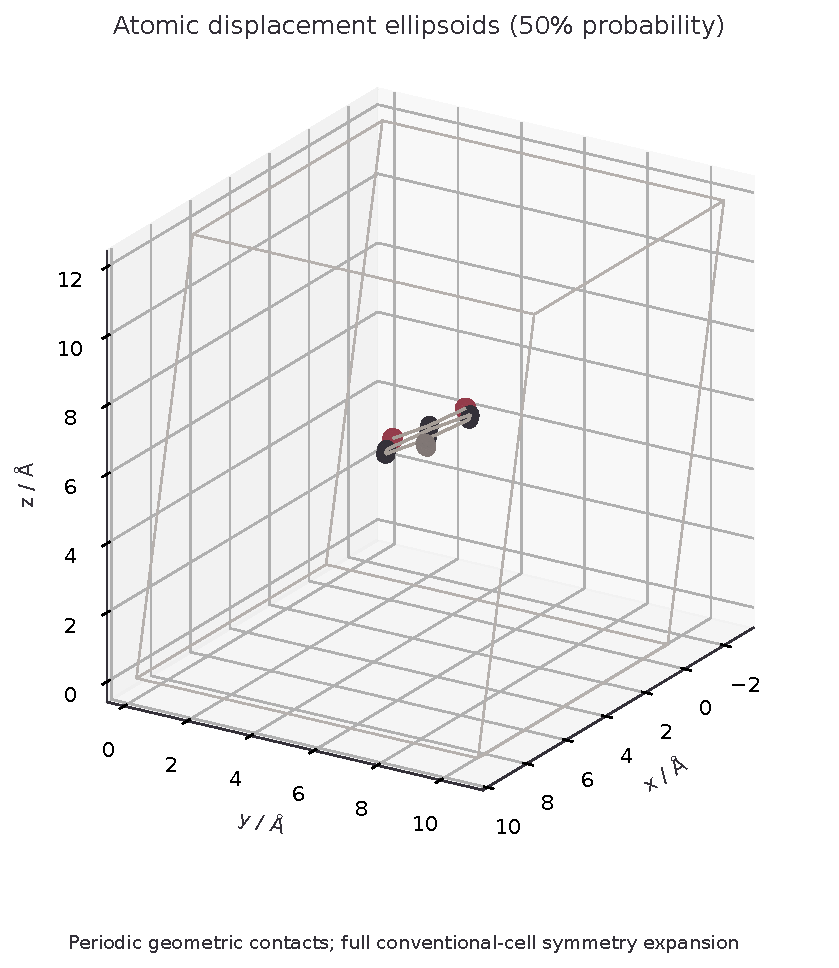
\includegraphics[width=.78\textwidth]{figures/structure_ellipsoids.pdf}
\caption{含各向异性 Br 位点的合成示例之 50\% 位移椭球。晶胞按真实非正交矩阵绘制；图中连接按元素半径与距离生成几何接触候选，不代表独立的化学键价判定。该图对应附录中的有噪声示例，并非实验结构。}
\end{figure}

\section{CIF 张量到笛卡尔张量}
CIF 与 SHELX 常将位移指数写作~\cite{cif_u}
\begin{equation}
T_h=\exp\left[-2\pi^2h^{\mathsf T}\mat D\mat U_{\mathrm{CIF}}\mat D h\right],
\qquad \mat D=\diag(|a^*|,|b^*|,|c^*|).
\end{equation}
因为 $\vct g=\mat A^{-\mathsf T}h$，与式~\eqref{eq:dw} 比较可得
\begin{equation}
\mat U_{\mathrm{cart}}=\mat A\mat D\mat U_{\mathrm{CIF}}\mat D\mat A^{\mathsf T}.
\label{eq:ucif}
\end{equation}
在斜晶胞中，直接把文件中的 $U_{ij}$ 当作笛卡尔协方差来画椭球，会同时改变方向和大小。实现通过不同反射的二次型保持不变来验证式~\eqref{eq:ucif}。

\section{常规差值电子密度}
给定精修模型和强度尺度 $k$，定义显示用幅度
\begin{equation}
F_{o,h}=\sqrt{\max(y_h/k,0)},\qquad
u_h=\begin{cases}F_{c,h}/|F_{c,h}|,&|F_{c,h}|>0,\\1,&|F_{c,h}|=0.\end{cases}
\end{equation}
常规无权重差值图与 $2F_o-F_c$ 图的系数为
\begin{equation}
C_h^{\Delta}=(F_{o,h}-|F_{c,h}|)u_h,
\qquad
C_h^{2o-c}=(2F_{o,h}-|F_{c,h}|)u_h.
\end{equation}
这些图使用模型相位，因此会带有相位偏倚。它们不是模型独立的密度测量，也不是含 $m$、$D$ 或 $\sigma_A$ 权重的统计最优地图。零级系数未知时取零会使显示图的平均密度为零；这一选择影响基线，不改变非零频率提供的结构信息。

精修使用的异常散射复系数一般不严格满足实密度的 Hermitian 条件。为生成实标量图，显示模块平均 $C_h$ 与 $C_{-h}^*$。这一处理仅用于地图，不合并或更改精修中的 Friedel 强度。完全重叠孪晶的观测强度也不属于单一振幅，因而默认不由其平方根直接生成差值密度；需要先有经过验证的去孪晶方案。

\section{从网格到等值面}
三维网格存储分数坐标采样。等值面算法在网格坐标中寻找与给定密度阈值的交点，再将网格位置 $\vct n$ 转为
\begin{equation}
\vct x=\diag(N_1^{-1},N_2^{-1},N_3^{-1})\vct n,
\qquad \vct r=\mat A\vct x.
\end{equation}
对斜晶胞，$\mat A$ 包含剪切和轴间夹角，不能用三个独立的轴长度相乘代替。实现为周期面追加首层切片，再作 marching cubes；追加切片之后，分母仍使用原始 $N_i$，否则整个晶胞会被人为收缩。

\begin{figure}[htbp]
\centering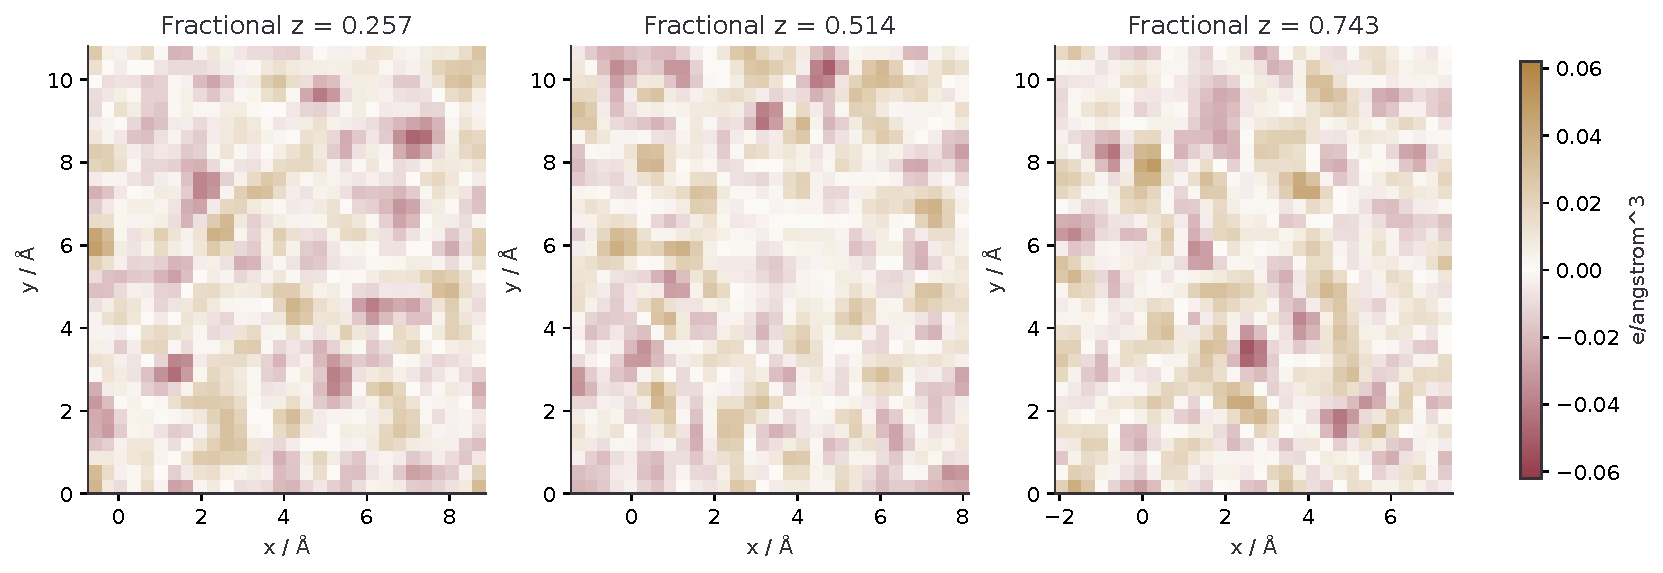
\includegraphics[width=\textwidth]{figures/density_sections.pdf}
\caption{合成示例的差值密度切片。色条给出实际密度单位；默认地图仅使用工作反射。切片和等值面不修改原始观测，缺失系数在显示地图中为零。}
\end{figure}

\section{倒易空间与统计诊断}
倒易空间点应画在 $\vct g_h=\mat B h$，而不是直接把 $h,k,l$ 当作欧氏坐标。颜色可编码标准化残差
\begin{equation}
z_h=\frac{y_h-\mu_h}{\sigma_h}.
\end{equation}
它能显示异常是否集中在特定倒易方向、分辨率范围或反射组。异常点只是需检查的候选，绘图不会自动删除它们。

\begin{figure}[htbp]
\centering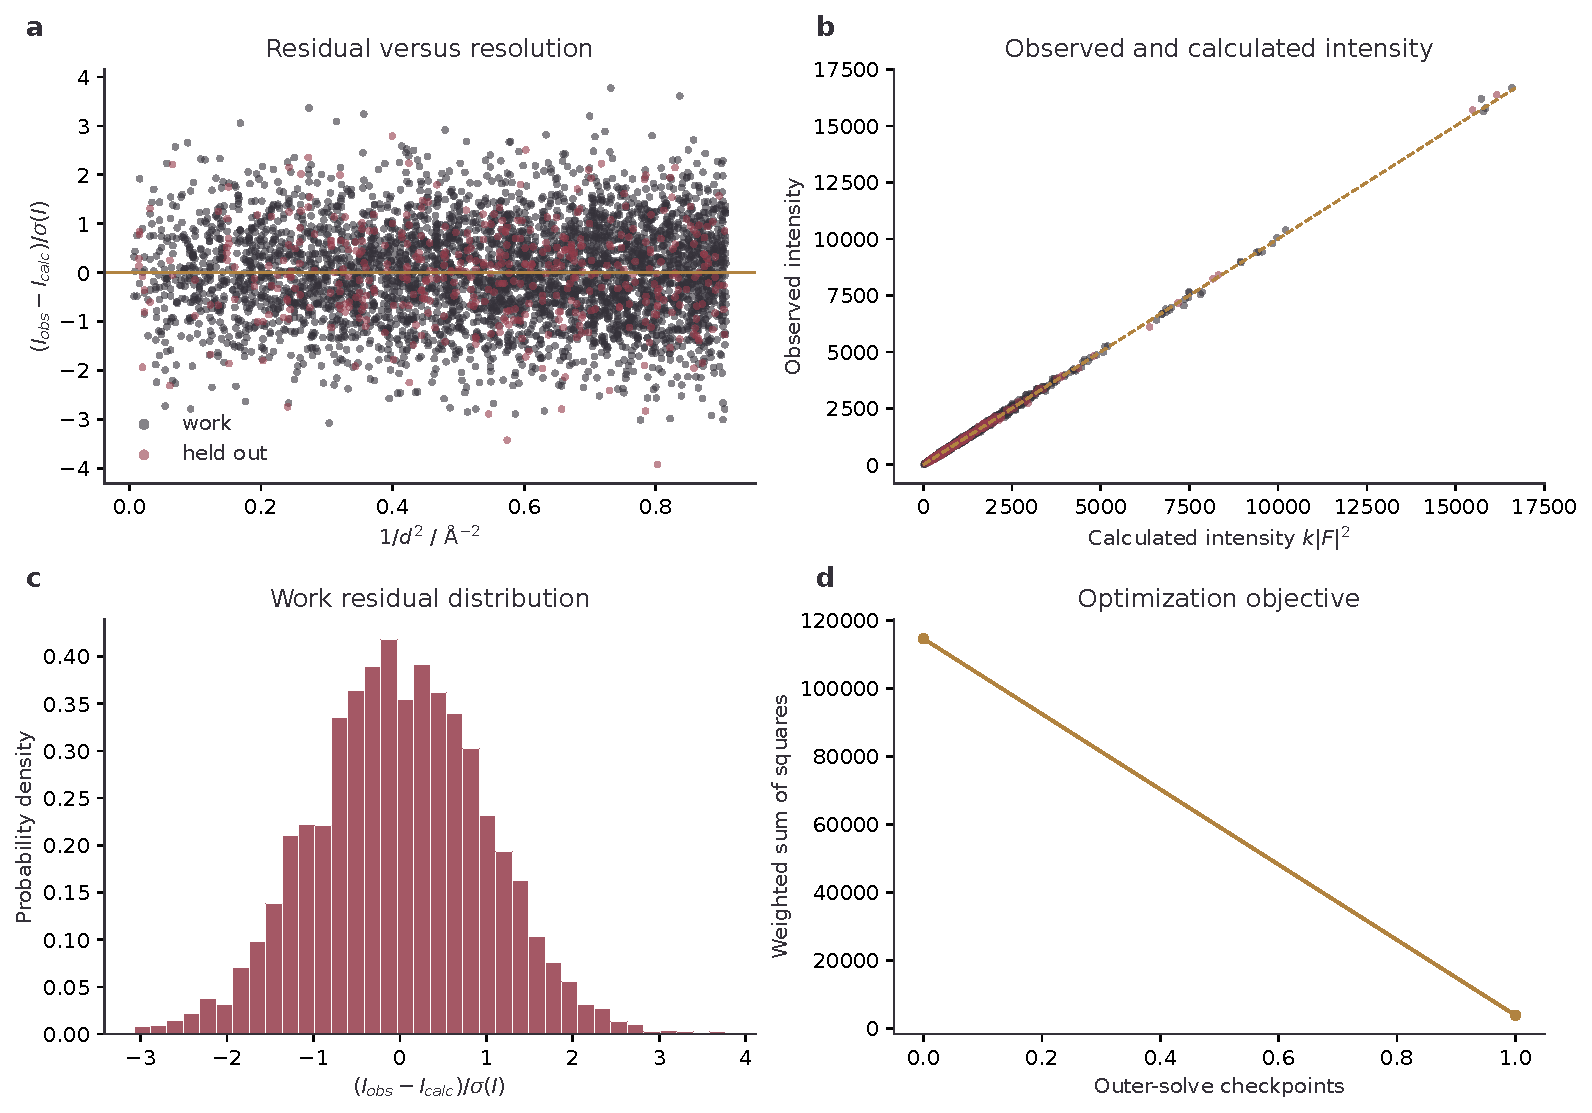
\includegraphics[width=\textwidth]{figures/refinement_diagnostics.pdf}
\caption{有噪声合成示例的强度一致性、分辨率依赖、残差分布及求解检查点。检查点记录初始状态和外层权重求解结束状态，并非每一次内部信赖域迭代。}
\end{figure}

参数相关图采用
\begin{equation}
R_{ij}=\frac{C_{ij}}{\sqrt{C_{ii}C_{jj}}}.
\end{equation}
它反映当前独立参数化下的局部相关。对 Cholesky 或 logit 变量，应结合参数名解释，不能将其直接称为原子笛卡尔坐标之间的相关图。秩亏时不绘制一个由伪逆伪装成的完整参数相关矩阵。

\section{交互图与可发表输出}
交互 HTML 在一个文件中嵌入绘图库，可离线旋转结构、查看原子属性、检查 Miller 指数与密度表面。静态输出采用 SVG 和 PDF 矢量格式，用于报告和论文排版。两者由相同的坐标、张量和数值结果生成，避免交互界面与最终图稿使用不同的科学数据。

绘图的可读性以明确信息为目标：椭球标明概率，地图标明类型和单位，反射图保留指数，合成数据标明来源。更多颜色和表面并不会增加证据；一张图应明确回答一个结构或模型诊断问题。

\chapter{从数学模型到可维护实现}
\section{数据层保持科学约定}
程序以四个核心对象组织计算。\code{Cell} 保存晶胞和度量，\code{Atom} 保存物理占有率、分数坐标和位移张量，\code{Structure} 保存原子与对称操作，\code{Reflections} 保存观测、标准差、批次和留出标志。对象建立时检查维度、有限数值、元素、唯一原子标签和物理范围。

内部约定稳定后，CIF、SHELX 与 JSON 之间的差异集中在输入输出边界。JSON 保存完整浮点精度及明确字段。传统 HKLF4 的固定列宽可能限制输出精度，因而精确往返使用 JSON；HKLF4 导出不会暗中把无法表达的留出标志丢失。

\section{模块对应的数学职责}
\begin{longtable}{p{43mm}p{93mm}}
\toprule 模块 & 数学或执行职责\\\midrule\endfirsthead
\toprule 模块 & 数学或执行职责\\\midrule\endhead
\code{model.py} & 晶胞矩阵、度量、周期最近像、物理数据对象\\
\code{symmetry.py} & 空间群操作、特殊位置、消光与候选诊断\\
\code{scattering.py} & 原子散射因子、对称展开、热位移、非相干畴强度\\
\code{phasing.py} & 带随机种子的 $P1$ 电荷翻转与稀疏原子投影\\
\code{refinement.py} & 参数化、信赖域估计、冻结权重、秩与协方差\\
\code{restraints.py} & 几何和位移限制残差\\
\code{absolute.py} & 显式异常散射因子与反射对商量分析\\
\code{maps.py} & 统一 Fourier 约定的密度、差值与 Patterson 图\\
\code{visualization.py} & 概率椭球、等值面、倒易空间、矢量图与离线交互图\\
\code{validation.py} & 反射轨道留出与观测诊断\\
\code{feedback.py} & 有信息上限的结构先验轮廓分解\\
\code{io.py}, \code{shelx.py} & 结构与反射格式转换、原始指令的无损保存\\
\code{compat.py} & 单独安装的官方程序执行、附属文件与运行记录\\
\code{agent.py}, \code{cli.py} & 结构化动作、输入快照、运行目录与机器结果\\
\code{mcp_server.py} & 官方 MCP SDK 适配层\\
\bottomrule
\end{longtable}
模块之间通过显式对象和返回值通信。相位恢复不调用语言模型，精修不修改原始反射，绘图不决定删点，兼容层不偷偷代替原生算法。该边界使单个数学部件可以独立测试与替换。

\section{复杂度与实际优化方向}
设独立反射数为 $H$，展开后的原子位置数为 $N$。直接结构因子求和的主要计算量为 $O(HN)$。对于 $P$ 个独立参数，三点差分构造完整 Jacobian 约需 $2P$ 次扰动计算，故一次完整导数评估的量级为 $O(PHN)$。密集法矩阵的分解约为 $O(P^3)$。

这说明大型 MOF 的性能瓶颈不能单靠外层 agent 并行解决。直接有效的优化是缓存不随参数变化的晶胞与散射数组、实现解析或自动微分 Jacobian、利用约束稀疏性，并在独立相位试验或候选模型之间并行。GPU 可以加速数组运算，但主机与设备的数据复制、动态特殊位置处理和不必要的全矩阵构造仍会限制性能。

配套实现采用 NumPy 向量化、SciPy 求解和 Gemmi 表格及文件基础设施。它没有声称实现 GPU、稀疏 CGLS 或全解析 Jacobian，也没有用不同数据或不同收敛准则给出与官方程序的速度排名。性能评价应在相同硬件、相同数据、相同模型和相同接受标准下进行。

对体素总数 $M=N_1N_2N_3$，一次三维 FFT 的复杂度约为 $O(M\log M)$，多起点相位恢复的计算量与试验数和迭代数近似成正比。相位试验之间相互独立，适于并行；同一试验中的迭代则按前一步结果顺序推进。

\section{验证层次}
验证应逐层建立独立性。闭式量检验包括晶胞度量、单参数尺度和概率椭球；物理不变量包括原点平移强度不变、Friedel 对称及其异常散射破缺、对称等价反射、特殊位置多重性和张量变换；外部数值对照使用 Gemmi 的独立结构因子计算；工作流验证检查输入不变、求解后精修、真实数据回归与工具传输。

合成数据由被测正向模型生成时，反演恢复能够检验工作流和优化，但不能独自证明正向模型正确。因此，需要外部实现、解析结果与真实观测三种证据互相补充。附录明确列出每项验证的来源与所能支持的结论。

\section{完整功能迁移的验收原则}
SHELXT 与 SHELXL 的功能由大量文件约定、默认值和数值分支共同组成。重新实现某个公式，不等于复现某条完整指令。一个可靠迁移单元应同时给出：输入语法与默认值；参数的数学定义；原生执行结果；异常和边界行为；与公开归档或官方程序的对照证据。

因此，本项目为官方指令建立逐项状态，而不是一个总体“兼容”布尔值。当前原生范围由源码与测试确定；原始指令文件保持不变并可交给官方程序。以后某个功能完成独立实现和对照测试后，才能将其从外部执行迁入原生能力表。

结构精修的成熟还需要跨化学体系的数据集，包括轻原子、重原子、手性、低完整度、强吸收、伪对称、无序、不同孪晶类型和大晶胞。对这些任务的覆盖，应以可复现样本和失败模式积累，而不是把一次成功求解外推为普遍等价性。

\appendix
\titleformat{\chapter}[display]{\Large\bfseries\color{ink}}{\large 附录\thechapter}{8pt}{\Huge}
\chapter{功能范围与互操作约定}
\label{app:capabilities}
\section{原生算法与官方执行路径}
交付版本为 Ariadne-Xtal 0.1.0。该名称表示独立实现，不表示 SHELX 官方分支。原生程序已经具有实际散射、相位恢复和精修能力；它尚不是保留所有 SHELXT/SHELXL 行为的独立替代品。官方执行路径要求使用者单独安装相应程序，源码包不包含其二进制或源代码。

\small
\begin{longtable}{p{31mm}p{57mm}p{44mm}}
\toprule 功能 & 原生行为 & 其余行为\\\midrule\endfirsthead
\toprule 功能 & 原生行为 & 其余行为\\\midrule\endhead
晶胞与空间群 & 任意有效晶胞、Gemmi 群表、显式操作、特殊位置 & 不等于自动空间群求解\\
相位恢复 & 已知组成的 $P1$ 电荷翻转与原子投影 & SHELXT 联立空间群、原点与元素赋值由官方路径执行\\
散射 & IT92 X 射线、各向同性与各向异性、显式色散 & 中子、电子及其他表不原生实施\\
精修 & 全部工作 $F^2$、尺度、坐标、ADP、指定占有率 & 完整 L.S./CGLS/BLOC 及所有默认值不等价\\
严格约束 & 特殊位置、原点、同坐标、同 ADP、同占有率、占有率和 & 全部自由变量与 AFIX/HFIX 指令由官方路径执行\\
限制 & 距离、角度、相似距离、平面、ADP 相似、标量刚键、各向同性 & 完整 RIGU、SAME、CHIV、SUMP 等原语未全部实施\\
孪晶 & 度量相容整数律的完全重叠畴，反演孪晶 & 一般 HKLF5 重叠组由官方路径执行\\
绝对结构 & 反演分数与固定模型商量估计 & 不等价于全部官方绝对结构统计\\
其他散射校正 & 不隐式加入 & EXTI、SWAT、ABIN、溶剂掩膜由官方路径执行\\
地图与绘图 & 密度、差值、Patterson、CCP4、概率椭球、离线交互、SVG/PDF & 未实施统计加权地图或通用去孪晶地图\\
文件 & JSON、结构 CIF、HKLF4、受支持 INS/RES 结构子集 & 完整原始 INS/RES 无损保留并交给官方程序\\
agent 接口 & Python、CLI、JSONL、MCP、输入快照和机器结果 & 宿主 LLM 策略独立于数值内核\\
结构反馈 & 高斯轮廓分解数值部件与先验信息上限 & 原始图像处理与完整闭环调度不在本包中\\
\bottomrule
\end{longtable}
\normalsize

\section{完整指令清单的含义}
\code{shelx_instruction_matrix.json} 与 \code{docs/COMPATIBILITY.md} 覆盖公开官方索引的 77 个指令名称~\cite{shelxl_instructions}，逐项标记词法识别、原文保存、原生结构转换和官方原样传递。表中的“原文保存”不是“指令已原生执行”，“官方传递”也不是“已验证数值等价”。

原生读取常见结构字段，例如 CELL、LATT、SYMM、命名 SFAC、DISP 及原子行。遇到没有完整翻译的 WGHT、TWIN、AFIX、HFIX、约束或精修控制等科学指令时，它明确拒绝原生转换。用户可以保留完整原始文件选择官方执行，也可以自行确认后建立含明确选项的原生 JSON 模型。

\section{SHELX 文件中的特别约定}
固定参数、自变量链接、特殊位置占有因子、$U_{ij}$ 次序和波长相关色散都影响科学含义。原生占有率始终是物理比例；RES 导出显式写出 DISP，包括零色散，防止另一个程序使用其默认表时产生未声明的差异。

含非零 ZERR 的原生转换会拒绝，因为当前结构精修不传播晶胞不确定度。CIF 的结构导入也不自动执行其内嵌精修指令。保持完整历史配方时，应使用原始文件及官方路径，而不是从坐标表重新构造一份看似相同的输入。

\section{官方后端的可复现执行}
执行器将 INS/RES、HKL、FAB、嵌套 include 与明确指定的附属文件复制到新的目录，记录输入和输出哈希，保存标准输出与错误输出，并在超时时终止进程组。原始源目录不被改写。

本次没有运行真实官方 SHELXT/SHELXL。兼容执行测试使用明确标识的模拟可执行程序，检验参数传递、字节保存、附属文件、退出码和超时。它们验证的是执行通道；原生数值的证据来自解析测试、Gemmi 对照、合成恢复与公开 FeN$_4$ 数据，而不是官方二进制一致性对照。

\chapter{验证数据与可复现实验}
\label{app:validation}
\section{自动化测试}
本次验证运行的 137 项测试全部通过，包含真实 MCP 标准输入输出初始化、工具列举和调用，未跳过该传输测试。运行使用 Python 3.12、NumPy 2.3.5、SciPy 1.17.0、Gemmi 0.7.5、Matplotlib 3.10.8、Plotly 7.1.0、scikit-image 0.26.0 和 MCP SDK 2.3.0。

测试包括晶胞和距离的解析或独立计算、六类空间群的结构因子对照、230 个参考空间群的系统消光、特殊位置与张量、异常散射、负强度、各种参数化、秩缺失、反射分组、格式往返、Fourier 地图、概率椭球和运行记录。测试通过表示这些明确断言成立，不意味着所有可能结构或官方指令都已被覆盖。

\begin{lstlisting}
python -m pip install -e ".[dev,mcp]"
ARIADNE_MCP_STDIO_TEST=1 python -m pytest -q
python -m ruff check src tests
\end{lstlisting}
MCP 传输测试需要运行环境允许本地进程和事件循环通信；默认测试将该项作为可选项。本次已经在允许相应通信的环境中实际执行。没有使用外部 LLM 账号或远程模型调用来替代传输测试。

\section{解析与独立实现对照}
单参数尺度检验使用式~\eqref{eq:scaleclosed}，负强度参与分子求和，结果及标准不确定度应与优化器一致。特殊位置检验对唯一对称位置求和，防止多重计数。张量检验比较式~\eqref{eq:ucif} 转换前后的散射指数。Fourier 检验用单个已知位置和直接求和检验峰方向、体积归一化和周期边界。概率椭球检验直接回代式~\eqref{eq:ellipsoid}。

Gemmi 独立结构因子计算用于检验原生求和，包括非正交晶胞与各向异性位移。Gemmi 同时提供本实现使用的标准表格，因此这些对照能检验求和、变换和约定，但不能独立验证散射表本身。散射表采用公开标准数据~\cite{gemmi_scattering,gemmi_symmetry}。

\section{从幅度到坐标的完整合成恢复}
四个碳原子置于 $a=5.2$、$b=5.7$、$c=6.1\,\angstrom$ 的正交 $P1$ 晶胞中，分数坐标为
\begin{equation}
\begin{pmatrix}
0.113&0.239&0.337\\
0.371&0.628&0.793\\
0.725&0.159&0.563\\
0.842&0.771&0.188
\end{pmatrix},\qquad U_{\mathrm{iso}}=0.012\,\angstrom^2.
\end{equation}
使用 4540 条合成反射，选择条件为 $d>0.55\,\angstrom$。未叠加随机噪声，$\sigma=0.2$ 仅用于目标尺度。求解器只接收晶胞、四个碳元素、强度和标准差，不接收真值坐标。随机种子为 1729，共 4 个起点，每个 400 次迭代。

\begin{table}[htbp]\centering\small
\begin{tabular}{rrrr}
\toprule 候选 & 精修前 RMS/$\angstrom$ & 精修后 RMS/$\angstrom$ & 精修后 $wR_2$\\\midrule
1&0.015254&$1.56\times10^{-16}$&$1.36\times10^{-15}$\\
2&0.013536&$4.00\times10^{-16}$&$1.44\times10^{-15}$\\
3&0.011407&$5.99\times10^{-16}$&$1.46\times10^{-15}$\\
4&0.010608&$8.69\times10^{-17}$&$1.33\times10^{-15}$\\
\bottomrule
\end{tabular}
\caption{同一合成数据的四个相位起点。RMS 在共同原点平移、反演与同元素原子排列优化后计算。}
\end{table}
这项实验验证了该实例的求解与精修链路。机器精度级残差来自无噪声数据和匹配的正向模型，不能解释为实验坐标精度，更不能外推为复杂结构的解析成功率。复现脚本为 \code{validation/run_phasing_recovery.py}，全部输入、候选和结果一并提供。

\section{有噪声数据与未参与拟合的反射}
交互绘图示例是一个明确标识的合成重原子模型，包含 10 个原子和非正交晶胞，其中 Br 采用各向异性位移。4446 条反射按固定种子产生独立高斯噪声，标准差为
\begin{equation}
\sigma_h=\sqrt{4+I_h^{\mathrm{true}}}+0.01I_h^{\mathrm{true}}.
\end{equation}
按对称与 Friedel 轨道预先留出 446 条，4000 条用于拟合，共 43 个独立参数。所得工作集 $R_1=0.018754$、$wR_2=0.046004$、$S=0.992143$；留出集 $wR_2=0.043572$。Jacobian 秩为 43/43。该示例演示输入快照、独立分组、精修、地图和离线绘图的完整调用，数据生成脚本与种子均包含在源码包内。

\section{公开 \texorpdfstring{FeN$_4$}{FeN4} 实测数据重新精修}
公开实验来自 Bykov 等人的 FeN$_4$ 研究~\cite{fen4_2018}。原始数据为高压单晶衍射，归档结构属于 $P\bar1$，不对称单元含 3 个原子，其中 Fe 位于反演中心。验证使用归档结构因子 CIF 中的 71 个实测 $F^2$ 与标准差；没有把同文件中的计算强度列作为观测。

采用归档给出的各向同性位移模型、显式异常散射修正和权重 $a=0.0282$、$b=0.3122$；晶胞使用结构因子文件中保留更多小数位的数值。Fe 坐标由反演中心固定，其他位置、各向同性位移与尺度构成 10 个独立参数。

\begin{table}[htbp]\centering\small
\begin{tabular}{lrr}
\toprule 指标 & 原生重新精修 & 公开归档值\\\midrule
$R_1[I>2\sigma(I)]$ & 0.04031574947 & 0.0403\\
$R_1$，全部反射 & 0.04126821960 & 0.0413\\
$wR_2$ & 0.08148047295 & 0.0815\\
拟合优度 $S$ & 1.183324413 & 1.183\\
Jacobian 秩/参数数 & 10/10 & 10 个参数\\
\bottomrule
\end{tabular}
\caption{原生精修复现公开归档指标的报告精度。相同的公开观测用于两列指标；本次未运行官方二进制程序。}
\end{table}
将初始 N 坐标扰动约 0.02 个分数坐标，并改变一个位移参数后，再次精修所得坐标与第一结果最大相差约 $5.1\times10^{-10}$。这说明该实例的结果不是单纯读取归档坐标或残差数值，而是通过重新优化恢复。

\begin{figure}[htbp]
\centering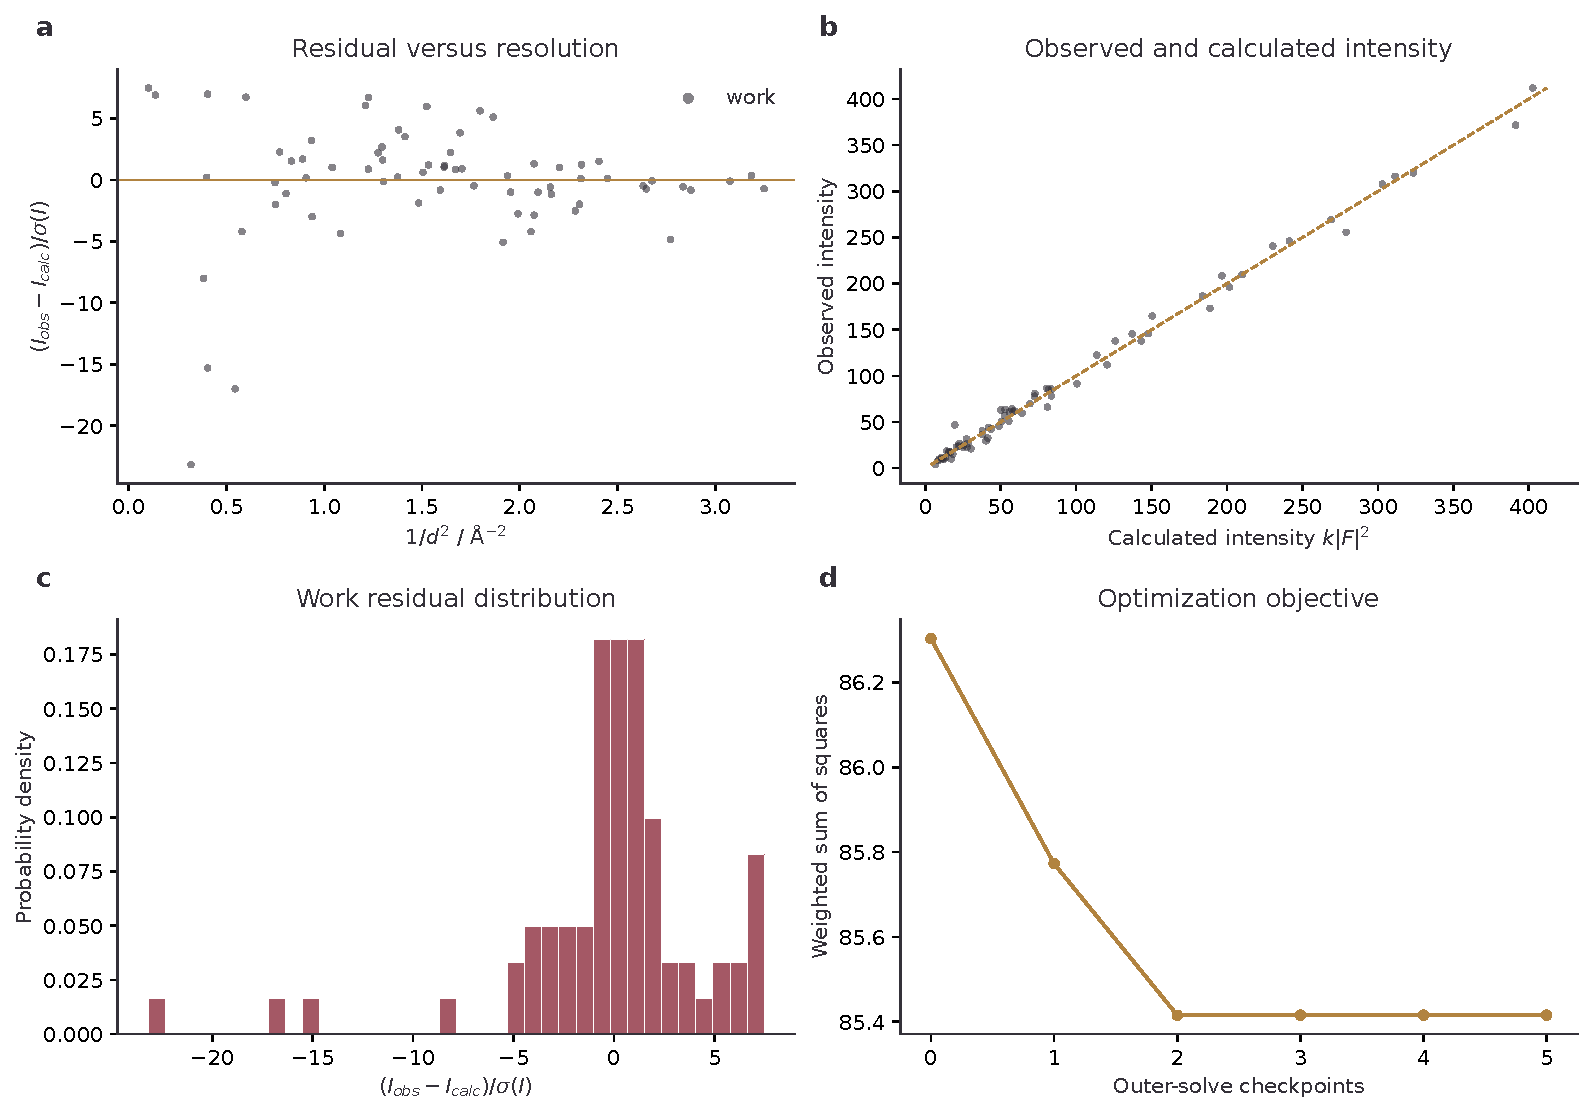
\includegraphics[width=\textwidth]{figures/fen4_refinement_diagnostics.pdf}
\caption{FeN$_4$ 的公开实测数据诊断。该例检验已知结构的精修，不构成从零求相位、运行速度或全部化学体系的基准。}
\end{figure}

原始 CIF、反射 CIF、文章引用、下载来源、许可说明与 SHA-256 均位于 \code{validation/public_data/}。脚本 \code{validation/run_real_fen4.py} 明确选择实测列、晶胞精度和权重，并保存完整机器结果。

\section{验证结论的适用范围}
当前证据支持：所列核心数学约定一致；已测例中的结构因子与约束精修正确；公开 FeN$_4$ 指标可复现；指定 $P1$ 合成结构能从幅度恢复；agent 请求可归档并通过实际 MCP 传输执行。尚没有开展完整官方二进制对照、多化学体系成功率研究或与 SHELXT/SHELXL 的等条件速度比较。上述验证与能力表共同界定本次交付，而不互相替代。

\chapter{安装、复现与扩展入口}
\section{最小安装与示例}
在解压后的项目目录中执行：
\begin{lstlisting}
python -m venv .venv
# macOS / Linux:
source .venv/bin/activate
# Windows PowerShell:
# .venv\Scripts\Activate.ps1
python -m pip install -e ".[dev,mcp]"
ariadne-xtal capabilities
ariadne-xtal run examples/refine_job.json --root .
\end{lstlisting}
示例数据已经包含在包内。重新生成时运行 \code{python examples/generate_examples.py}。每次任务在 \code{runs/} 下创建一个新目录；实际目录名由返回的 JSON 给出。

原生结构模型与反射 JSON 分别保存，示例请求为
\begin{lstlisting}
{
  "action": "refine",
  "structure": "examples/demo_start.json",
  "hkl": "examples/demo_reflections.json",
  "options": {
    "max_nfev": 150,
    "covariance_scale": "absolute"
  },
  "graphics": true
}
\end{lstlisting}
输入中保留反射的 \code{free_flags}，不需要从批次符号推断。全部字段定义见 \code{docs/API.md}。

\section{Python 精修接口}
\begin{lstlisting}
from ariadne_xtal.io import read_structure, read_reflections
from ariadne_xtal.refinement import RefinementOptions, refine

model = read_structure("examples/demo_start.json")
data = read_reflections("examples/demo_reflections.json")
result = refine(
    model, data,
    options=RefinementOptions(max_nfev=150),
    restraints=[],
    constraints=[],
)
print(result.metrics)
print(result.warnings)
\end{lstlisting}
结构求解接口为 \code{solve_p1(cell, reflections, elements, options)}；已知组成必须对应 $P1$ 单胞内原子数。对称结构的独立原子列表与完整单胞列表不可混用。

\section{连接宿主智能体}
JSONL 入口适合逐条请求：
\begin{lstlisting}
ariadne-xtal serve --root /absolute/path/to/project
\end{lstlisting}
标准输入每行是一个 JSON 请求，标准输出每行是一个结构化结果。MCP 入口为
\begin{lstlisting}
ariadne-xtal-mcp --root /absolute/path/to/project
\end{lstlisting}
宿主可调用 \code{crystal_capabilities} 查询能力，再用 \code{crystal_execute} 执行请求。运行 MCP 不需要把语言模型凭据写进本项目；宿主自行管理模型与对话。

\section{选择官方后端}
先在本机按官方要求安装程序，再显式提供可执行文件：
\begin{lstlisting}
ariadne-xtal run legacy_job.json --root . \
  --shelxl /absolute/path/to/shelxl
\end{lstlisting}
\begin{lstlisting}
{
  "action": "legacy",
  "engine": "shelxl",
  "input": "data/sample.ins",
  "timeout": 300
}
\end{lstlisting}
\code{data/sample.hkl} 与相应附属文件应位于输入目录。未在启动时启用该引擎，任务即被拒绝。结构求解可用相同方式明确选择 \code{shelxt}。官方程序的授权与安装不由此源码包替代~\cite{shelx_distribution}。

\section{复现报告与数值验证}
\begin{lstlisting}
python validation/run_real_fen4.py
python validation/run_phasing_recovery.py
python tools/fetch_report_fonts.py
cd docs
xelatex -interaction=nonstopmode -halt-on-error report.tex
xelatex -interaction=nonstopmode -halt-on-error report.tex
\end{lstlisting}
报告的所有公式保留为 LaTeX；矢量图在 \code{docs/figures/} 中。中文字体可使用系统已安装的 Noto Serif CJK SC，也可由脚本从官方字体仓库下载。字体文件未打入源码包，随下载保存其许可。程序测试不依赖排版系统。

\section{扩展一个原生计算模块}
新模块首先明确数据对象、物理单位、优化变量和可辨识条件；随后给出独立的解析或外部数值检验，再加入公开数据回归。工具层新增动作时定义专属输入字段和资源预算，并把新能力写入机器可读能力表。若该模块迁移一条原始 SHELXL 指令，还需要验证默认值、选取语法、文件回写和与其他指令的相互作用。

本报告中的推导、源码模块、验证输入和运行清单构成同一套可检查的计算说明。修改算法时，应同步更新对应公式、接口边界与复现实验，使结构结论始终能追溯到其观测与计算定义。

\backmatter
\begin{thebibliography}{99}
\addcontentsline{toc}{chapter}{参考文献}
\latinfont
\bibitem{shelxt2015} Sheldrick, G. M. SHELXT---Integrated space-group and crystal-structure determination. \textit{Acta Crystallographica A} \textbf{71}, 3--8 (2015). \href{https://doi.org/10.1107/S2053273314026370}{doi:10.1107/S2053273314026370}.
\bibitem{shelxl2015} Sheldrick, G. M. Crystal structure refinement with SHELXL. \textit{Acta Crystallographica C} \textbf{71}, 3--8 (2015). \href{https://doi.org/10.1107/S2053229614024218}{doi:10.1107/S2053229614024218}.
\bibitem{shelxl_instructions} SHELX. Alphabetical list of SHELXL instructions. \url{https://shelx.uni-goettingen.de/shelxl_html.php}. Accessed 30 October 2026.
\bibitem{chargeflip2004} Oszl\'anyi, G. and S\"ut\H{o}, A. Ab initio structure solution by charge flipping. \textit{Acta Crystallographica A} \textbf{60}, 134--141 (2004). \href{https://doi.org/10.1107/S0108767303027569}{doi:10.1107/S0108767303027569}.
\bibitem{sayre1952} Sayre, D. The squaring method: a new method for phase determination. \textit{Acta Crystallographica} \textbf{5}, 60--65 (1952). \href{https://doi.org/10.1107/S0365110X52000137}{doi:10.1107/S0365110X52000137}.
\bibitem{direct_methods} IUCr. An introduction to direct methods. IUCr Teaching Pamphlets. \url{https://www.iucr.org/what-we-do/education/pamphlets/introduction-direct-methods}. Accessed 30 October 2026.
\bibitem{rigu2012} Thorn, A., Dittrich, B. and Sheldrick, G. M. Enhanced rigid-bond restraints. \textit{Acta Crystallographica A} \textbf{68}, 448--451 (2012). \href{https://doi.org/10.1107/S0108767312014535}{doi:10.1107/S0108767312014535}.
\bibitem{parsons2013} Parsons, S., Flack, H. D. and Wagner, T. Use of intensity quotients and differences in absolute structure refinement. \textit{Acta Crystallographica B} \textbf{69}, 249--259 (2013). \href{https://doi.org/10.1107/S2052519213010014}{doi:10.1107/S2052519213010014}.
\bibitem{fen4_2018} Bykov, M., Khandarkhaeva, S., Fedotenko, T., Sedmak, P., Dubrovinskaia, N. and Dubrovinsky, L. Synthesis of FeN$_4$ at 180 GPa and its crystal structure from a submicron-sized grain. \textit{Acta Crystallographica E} \textbf{74}, 1392--1395 (2018). \href{https://doi.org/10.1107/S2056989018012161}{doi:10.1107/S2056989018012161}. Original supporting data and attribution are retained in the source package.
\bibitem{gemmi_scattering} Gemmi developers. Scattering: form factors, anomalous scattering and direct summation. \url{https://gemmi.readthedocs.io/en/latest/scattering.html}. Accessed 30 October 2026; implementation tested with Gemmi 0.7.5.
\bibitem{gemmi_symmetry} Gemmi developers. Crystallographic symmetry and space-group operations. \url{https://gemmi.readthedocs.io/en/latest/symmetry.html}. Accessed 30 October 2026.
\bibitem{gemmi_grid} Gemmi developers. Grids and maps. \url{https://gemmi.readthedocs.io/en/latest/grid.html}. Accessed 30 October 2026.
\bibitem{cif_u} IUCr COMCIFS. Core CIF dictionary: \code{_atom_site_aniso_U_} definitions. \url{https://www.iucr.org/__data/iucr/cifdic_html/1/cif_core.dic/Iatom_site_aniso_U_.html}. Accessed 30 October 2026.
\bibitem{scipy_lsq} SciPy developers. \code{scipy.optimize.least_squares}: nonlinear least squares with bounds. \url{https://docs.scipy.org/doc/scipy/reference/generated/scipy.optimize.least_squares.html}. Accessed 30 October 2026; implementation tested with SciPy 1.17.0.
\bibitem{mcp_sdk} Model Context Protocol. Official Python SDK and server documentation. \url{https://github.com/modelcontextprotocol/python-sdk}; \url{https://py.sdk.modelcontextprotocol.io/}. Accessed 30 October 2026; stdio adapter tested with SDK 2.3.0.
\bibitem{shelx_distribution} SHELX distribution and registration information, linked by CCP4. \url{https://www.ccp4.ac.uk/download/shelx.php}; \url{https://shelx.uni-goettingen.de/}. Accessed 30 October 2026.
\end{thebibliography}

\end{document}
